 % Sayfa biçimi ve metin puntosu
\documentclass[a4paper,12pt]{report}
\usepackage[utf8]{inputenc}
\usepackage[english, turkish]{babel}

\usepackage{listings}

\usepackage{lineno}

% /////////////////////////////

\usepackage{marginnote} % Required for margin notes
\usepackage{wallpaper} % Required to set each page to have a background
\usepackage{lastpage} % Required to print the total number of pages
% \usepackage[left=1.3cm,right=4.6cm,top=1.8cm,bottom=4.0cm,marginparwidth=3.4cm]{geometry} % Adjust page margins
\usepackage{amsmath} % Required for equation customization
\usepackage{amssymb} % Required to include mathematical symbols
\usepackage{xcolor} % Required to specify colors by name
\usepackage[T1]{fontenc}
\usepackage[utf8]{inputenc}

\usepackage{fancyhdr} % Required to customize headers


%----------------------------------------------------------------------------------------
%	HEADER INFORMATION
%-------------------------------------------------------------------------------------

\fancyhead[L]{\begin{tabular}{l r | l r} % The header is a table with 4 columns
\textbf{Ağ Programlama} & Lab. Uygulamları & \textbf{Sayfa} & \thepage/\pageref{LastPage} \\ % Project name and page count
\textbf{Tarih}  & \today \\ % Job number and last updated date
\textbf{Dönemi} & 2022-2023 Bahar & \textbf{Tarih} &\today \\ % Version and reviewed date
\textbf{Ders Sor.} & Prof.Dr.Resul Daş & \textbf{Lab.Sor} & Arş.Gör. Oğuzhan Katar\\ % Designer and reviewer
\end{tabular}}

%-------------------------------------------------------------------------------------
% \begin{document}


% /////////////////////////////

% \usepackage{fancyhdr} % Required to customize headers


% \setcounter{secnumdepth}{4} % how many sectioning levels to assign numbers to
% \setcounter{tocdepth}{4}    % how many sectioning levels to show in ToC

\usepackage[absolute,overlay]{textpos}
\usepackage[document]{ragged2e}	%Sağa sola ve heriki yana yasla 
\usepackage{xcolor}	%renk paketi
\usepackage[top=3.0cm, bottom=2.5cm, left=3.25cm, right=2.5cm]{geometry} % Kenar boşlukları
\usepackage{textgreek} % Yunanca karakter 
\usepackage{titlesec} % Anabölüm ve alt bölüm başlıkları font ve boşluk değişimi
% \usepackage[final,dvips]{graphicx}
% \usepackage[pdftex]{graphicx}
\usepackage{graphicx}

% \usepackage{graphicx} 
% \usepackage{epstopdf}

% \usepackage{ifpdf}
% \ifpdf
%   \DeclareGraphicsExtensions{.pdf,.png,.jpg}
% \else
%   \DeclareGraphicsExtensions{.eps}
% \fi
% \usepackage{epstopdf}
% \DeclareGraphicsRule{.png}{.eps}{.bb}{.pdf}  %{pdf}{-crop.pdf}{`pdfcrop #1}
% /\DeclareGraphicsRule{.png}{eps}{.bb}{}
\usepackage[export]{adjustbox}



\usepackage{amsmath,amsfonts,amsthm,bm} % Denklem paketi 
\usepackage{lmodern}   
\usepackage{textcomp}
\usepackage{setspace}
\usepackage{indentfirst}
%\usepackage{csquotes}
\usepackage{textcmds}
\usepackage[unicode]{hyperref} %	Hiper link paketi
\hypersetup{hidelinks}
\usepackage{url}

\usepackage{tocloft} %	Tablo,Şekil, İçindekiler Sayfası ayarları
\usepackage[hypcap=false]{caption}
\usepackage{subcaption}
\usepackage{float}
%\usepackage{mhchem}
\usepackage{booktabs} %	Tablo alt çizgi kalınlığı ayarı
\usepackage{tikz} %	Tik sembolü ekleme
\usetikzlibrary{mindmap,trees,shapes.geometric,arrows,automata,petri,positioning}
\usepackage{minted}

\usepackage{enumitem}
\usepackage{appendix}
%\usepackage{biblatex}
\usepackage{secdot}
\usepackage{verbatim}
% \newtheorem{definition}{Tanım}[section]
% \newtheorem{problem}{Problem}[section]
% \newtheorem{example}{Örnek}[section]
% \newtheorem{algorithm}{Algoritma}[section]
\usepackage{xpatch}
\makeatletter
\AtBeginDocument{\xpatchcmd{\@thm}{\thm@headpunct{.}}{\thm@headpunct{}}{}{}}
\makeatother
\usepackage[section]{placeins}

\usepackage{multicol}

\DeclareTextCompositeCommand{\.}{T1}{i}{\accent"0A \i} %i sorunu için
%----------------------------------------------------------------------------------------------------
%	Alttaki blok kalın büyük-küçük (bold small caps) fontu 
%	oluşturmayı amaçlar 
\RequirePackage{fix-cm}
\usepackage[T1]{fontenc}
\usepackage{lmodern}
\rmfamily
\DeclareFontShape{T1}{lmr}{b}{sc}{<->ssub*cmr/bx/sc}{}
\DeclareFontShape{T1}{lmr}{bx}{sc}{<->ssub*cmr/bx/sc}{}
%----------------------------------------------------------------------------------------------------
%----------------------------------------------------------------------------------------------------

%----------------------------------------------------------------------------------------------------
%	Alttaki blok matematik denklemlerinin 1cm girdi biçimde sola hizlanmasını amaçlar 
\makeatletter
\newcommand{\mathleft}{\@fleqntrue\@mathmargin1cm}
\newcommand{\mathcenter}{\@fleqnfalse}
\makeatother
%----------------------------------------------------------------------------------------------------
%----------------------------------------------------------------------------------------------------

\urlstyle{rm} %	url referans fontu değişimi (şaun kullanılan font roman )

\usepackage{longtable} %	Uzun tabloların bir sonraki sayfadan devam etmesini sağlar

%----------------------------------------------------------------------------------------------------
%	Alttaki blok metni belirli boyutlara sahip bir kutu içerisine sıkıştırmayı amaçlar 
\usepackage{environ}
\usepackage{relsize}
\makeatletter
\NewEnviron{fitbox}[2]{%
	\minipage{#1}%
	\sbox0{\minipage{#1}\strut\BODY\strut\endminipage}%
	\Gscale@div\factor{#2}{\dimexpr\ht0+\dp0\relax}%
	\relscale{\factor}%
	\BODY
	\endminipage
}
\makeatother
%---------------------------------------------------------------------------------
%----------------------------------------------------------------------------------------------------
% 	Sayfaya sığmayan kelimelerin "-" ile bölünmesini engelleyen kod bloğu
\tolerance=1
\emergencystretch=\maxdimen
\hyphenpenalty=10000
\hbadness=10000
%----------------------------------------------------------------------------------------------------
% ///////////////////////////////////////////////////////////////////////
% ENVIROMENT WILL BE USEFUL IN THE FUTURE
% ///////////////////////////////////////////////////////////////////////
% \newenvironment{sheet}
%     {\begin{center}
%     \begin{tabular}{|p{0.9\textwidth}|}
%     \geometry{
%         left=1.3cm,
%         right=4.6cm,
%         top=1.8cm,
%         bottom=4.0cm,
%         marginparwidth=3.4cm
%     }
    

% \setlength{\headheight}{80pt} % Increase the size of the header to accommodate meta-information
% \pagestyle{fancy}\fancyhf{} % Use the custom header specified below
% \renewcommand{\headrulewidth}{0pt} % Remove the default horizontal rule under the header

% \setlength{\parindent}{0cm} % Remove paragraph indentation
% \newcommand{\tab}{\hspace*{2em}} % Defines a new command for some horizontal space

% \newcommand\BackgroundStructure{ % Command to specify the background of each page
% \setlength{\unitlength}{1mm} % Set the unit length to millimeters

% \setlength\fboxsep{0mm} % Adjusts the distance between the frameboxes and the borderlines
% \setlength\fboxrule{0.5mm} % Increase the thickness of the border line
% \put(10, 10){\fcolorbox{black}{blue!10}{\framebox(155,247){}}} % Main content box
% \put(165, 10){\fcolorbox{black}{blue!10}{\framebox(37,247){}}} % Margin box
% \put(10, 262){\fcolorbox{black}{white!10}{\framebox(192, 25){}}} % Header box
% \put(175, 263){
\includegraphics[height=23mm,keepaspectratio]{00-images/00-logo.png}} % Logo box - maximum height/width: 
% }

%     \hline\\
%     }
%     { 
%     \\\\\hline
%     \end{tabular} 
%     \end{center}
% }
% \newenvironment{answer}{}{}
% ///////////////////////////////////////////////////////////////////////
% ENVIROMENT WILL BE USEFUL IN THE FUTURE
% ///////////////////////////////////////////////////////////////////////
% ///////////////////////////////////////////////////////////////////////
% CUSTOM LISTING STYLE FOR CODE SAMPLES
% ///////////////////////////////////////////////////////////////////////
% \definecolor{codegreen}{rgb}{0,0.6,0}
% \definecolor{codegreen}{rgb}{0.373, 0.596, 0.082}
\definecolor{keyword_green}{rgb}{0.027, 0.506, 0.004}

% #5f9815 green
% 8edffb blue
\definecolor{line_gray}{rgb}{0.5,0.5,0.5}
\definecolor{string_red}{rgb}{1, 0, 0}
\definecolor{comment_blue}{rgb}{0.318, 0.6, 0.745}
% #b42171 red
% \definecolor{backcolour}{rgb}{0.95,0.95,0.92}

\lstdefinestyle{code}{
    frame=lines,
    % backgroundcolor=\color{backcolour},   
    commentstyle=\color{comment_blue}\slshape,
    keywordstyle=\color{keyword_green}\bfseries,
    stringstyle=\color{string_red},
    numberstyle=\tiny\color{line_gray},
    basicstyle=\ttfamily\scriptsize,
    breakatwhitespace=false,         
    breaklines=true,                 
    captionpos=b,                    
    keepspaces=true,                 
    numbers=left,                    
    numbersep=5pt,                  
    showspaces=false,                
    showstringspaces=false,
    showtabs=false,                  
    tabsize=2
}
\lstset{style=code}
% ///////////////////////////////////////////////////////////////////////
% CUSTOM LISTING STYLE FOR CODE SAMPLES
% ///////////////////////////////////////////////////////////////////////
% ///////////////////////////////////////////////////////////////////////
% CUSTOM LISTING STYLE FOR CODE SAMPLES
% ///////////////////////////////////////////////////////////////////////
\usepackage{enumerate}		    % Enumerate Environments
\usepackage[framemethod=TikZ]{mdframed}
\usepackage{tikz, tabularx}

\mdfdefinestyle{exerciseStyle}{%
	frametitlerule=true,
	roundcorner=5pt,
	linecolor=black,
	outerlinewidth=0.5pt,
	middlelinewidth=0.5pt
}
\mdtheorem[style=exerciseStyle]{question}{\textbf{Soru}}



% ///////////////////////////////////////////////////////////////////////
% ///////////////////////////////////////////////////////////////////////

% \mdfdefinestyle{sheetStyle}{%
%     left=1.3cm,
%     right=4.6cm,
%     top=1.8cm,
%     bottom=4.0cm,
%     marginparwidth=3.4cm
% }
% \mdtheorem[style=sheetStyle]{sheet}{\textbf{Sheeeeeeeeeeet}}
% ///////////////////////////////////////////////////////////////////////
% ///////////////////////////////////////////////////////////////////////

% ///////////////////////////////////////////////////////////////////////
% CUSTOM LISTING STYLE FOR CODE SAMPLES
% ///////////////////////////////////////////////////////////////////////
%----------------------------------------------------------------------------------------------------
%	Sayfa numarası boşluğu
\usepackage{calc}
\setlength{\footskip}{\paperheight
	-(1in+\voffset+\topmargin+\headheight+\headsep+\textheight)
	-1.5cm}
%---------------------------------------------------------------------------------
%----------------------------------------------------------------------------------------------------
%	Sayfa numarası font değişimi
\usepackage{fancyhdr}
\fancypagestyle{plain}{%
	\fancyhf{} 
	\fancyfoot[C]{\fontsize{10pt}{10pt}\selectfont\thepage} 
	\renewcommand{\headrulewidth}{0pt}
	\renewcommand{\footrulewidth}{0pt}}
\pagestyle{plain}
%----------------------------------------------------------------------------------------------------
%----------------------------------------------------------------------------------------------------

\usetikzlibrary{graphs,graphs.standard}

\newcount\nodecount
\tikzgraphsset{
  declare={subgraph N}%
  {
    [/utils/exec={\global\nodecount=0}]
    \foreach \nodetext in \tikzgraphV
    {  [/utils/exec={\global\advance\nodecount by1}, 
      parse/.expand once={\the\nodecount/\nodetext}] }
  },
  declare={subgraph C}%
  {
    [cycle, /utils/exec={\global\nodecount=0}]
    \foreach \nodetext in \tikzgraphV
    {  [/utils/exec={\global\advance\nodecount by1}, 
      parse/.expand once={\the\nodecount/\nodetext}] }
  }
}
\usepackage{tabularx}
\usepackage{blkarray}
\usepackage{amsmath}
\usepackage{amssymb}
\usepackage{wrapfig}

\usepackage[printonlyused]{acronym} % Kısaltmalar

\begin{document}
%----------------------------------------------------------------------------------------------------
%	Büyük küçük yazı sitilinde "i" karakteri sorununun çözümü için
%	gerekli kod bloğu. Metin içerisinde büyük-küçük yazı sitilinde
%	"i" karekteri kullanmak için "\.\i" yazmanız gerekmektedir.
% \expandafter\let\csname\string\T1\string\.-\string\i\endcsname\relax
\shorthandoff{=}

%----------------------------------------------------------------------------------------------------
%----------------------------------------------------------------------------------------------------
% 	Latex dökümanınızı oluşturmadan önce ilk olarak "tezbilgileri.tex" dosyasına girerek
%						kendi metninize ait bilgileri giriniz! 
%	
%	"tezbilgileri.tex"  doyasındaki bilgilerin doğru bir biçimde girilmesi; pencere altı kapak, 
%	iç kapak, onay metni ve beyan metninin otomatik olarak doldurulmasını sağlayacaktır.
%	Herhangi bir problem yaşamadığınız takdirde "pencerealtikapak.tex", "ickapak.tex", "onay.tex"
%	"beyan.tex" dosyalarında herhangi bir değişiklik yapmayınız.

\def\antet{T.C.\newline \textsc{FIRAT ÜNİVERSİTESİ  \newline TEKNOLOJİ FAKÜLTESİ \newline YAZILIM MÜHENDİSLİĞİ BÖLÜMÜ}}

%----------------------------------------------------------------------------------------
%      TEZ BAŞLIĞI YAZIM ALANI
%----------------------------------------------------------------------------------------

\def\tezbasligi{Go Dili ile Ağ Programlama}

\def\tezbasligien{Network Progrramming with Go}


\def\tezyazari{Uğur FIRAT}   % tez yazarının Adı SOYADI

\def\derece{YMH455 Bitirme Projesi} % Yüksek Lisans/Doktora Tezi, Seminer Çalışması

\def\dereceen{Bachelor's Thesis} % Master's Thesis, Ph.D. Thesis veya Seminar Study


\def\abd{Yazılım Mühendisliği Bölümü}
\def\abden{Department of Software Engineering } % İngilizce Anabilim Dalını Giriniz...
%\def\bilimdali{........varsa.. Bilim Dalı}
%\def\program{..........varsa...Teknolojileri Programı}
%\def\programen{.....varsa..... Technologies Program}    % İngilizce Program ismi giriniz  

\def\yil{2022}
\def\ay{Haziran}
\def\ayen{June}

%----------------------------------------------------------------------------------------------------
%----------------------------------------------------------------------------------------------------
% DANIŞMAN, 2. DANIŞMAN, BAŞKAN ve ÜYE BİLGİLERİNİ GİRİNİZ
% KULLANMADIĞINIZ BÖLÜMLERİ PASİF KONUMA GETİRİNİZ
%----------------------------------------------------------------------------------------------------
%----------------------------------------------------------------------------------------------------

\def\danisman {Prof. Dr. Resul DAŞ}
\def\danismankurum{Fırat Üniversitesi, Teknoloji Fakültesi, Yazılım Mühendisliği} 
\def\danismankarar {Onayladım} % Oynaylamıyorum
\def\danismanikikarar {Onayladım} % Oynaylamıyorum

\def\baskan {Prof. Dr. }
\def\baskankurum{Fırat Üniversitesi, Teknoloji Fakültesi, Yazılım Mühendisliği} 
\def\baskankarar {Onayladım} % Oynaylamıyorum

\def\uyebir {Doç. Dr.}
\def\uyebirkurum{Fırat Üniversitesi, Teknoloji Fakültesi, Yazılım Mühendisliği} 
\def\uyebirkarar {Onayladım} % Oynaylamıyorum

%\def\uyeiki {Unvan Adı SOYADI }
%\def\uyeikikurum{Fırat Üniversitesi, Teknoloji Fakültesi, Yazılım Mühendisliği} 
%\def\uyeikikarar {Onayladım} % Oynaylamıyorum

%\def\uyeuc {Unvan Adı SOYADI }
%\def\uyeuckurum{............Üniversitesi, ......... Fakültesi} 
%\def\uyeuckarar {Onayladım} % Oynaylamıyorum

%\def\uyedort {Unvan Adı SOYADI - yoksa siliniz}
%\def\uyedortkurum{..........Üniversitesi, ......... Fakültesi} 
%\def\uyedortkarar {Onayladım} % Oynaylamıyorum

%\def\uyebes {Unvan Adı SOYADI - yoksa siliniz}
%\def\uyebeskurum{............Üniversitesi, .........Fakültesi} 
%\def\uyebeskarar {Onayladım} % Oynaylamıyorum


\def\sayfasayisi {\normalsize{xii + 70}} % Ön Bölüm sayfaları ve tez sayfa sayısı (Özgeçmiş hariçtir)

\def\itt{İlk Teslim Tarihi} % "23.08.2019" şeklinde giriniz. Tezin Enstitüye ilk teslim edildiği tarih. 
\def\st{Savunma Tarihi} % "23.08.2019" şeklinde giriniz.  


% \def\anahtarkelimeler{Örnek Kelime-1, Örnek Kelime-2, Örnek Kelime-3, Örnek Kelime-4}
\def\anahtarkelimeler{Go Programlama Dili, Golang, Soket Programlama, TCP/UDP, Ağ Uygulamaları.} % Üst satırdaki örneğe göre giriş yapınız.

\def\Keywords{Go Programming Language, Golang, Socket Programming, TCP/UDP, Network Applications.} % İngilizce Anahtar Kelimeleri giriniz...

%***********************************************************
%*********** Pencere Altı Kapak*****************************
%***********************************************************
\newgeometry{top=2.5cm, bottom=2.5cm, left=3.25cm, right=2.5cm}

\begin{titlepage}


\centering
\begin{small}
	\textbf{\antet\\}
\end{small}
\vspace*{14cm}





\begin{textblock*}{11cm}(5.5cm,18.0cm) % {block width} (coords) 

\begin{fitbox}{11cm}{7cm}
\begin{center}
\begin{normalsize}
\bfseries\tezbasligi\\ 
\end{normalsize}\vspace{0.35cm}
\end{center}


\begin{center}
{\small\textbf{\tezyazari}}
\vspace{0.7cm}\break
{\small\derece}
\vspace{0.5cm}\break
{\small{\footnotesize \abd}}
\vspace{0.1cm}\break
%{\footnotesize\program}
%\vspace{0.2cm}\break
%{\footnotesize\bilimdali}
%\vspace{0.35cm}\break
\ay \: \yil

\end{center}
\end{fitbox}
\end{textblock*}


\vspace{\stretch{0.5}}
\end{titlepage}
\restoregeometry
\newpage
%***********************************************************
%*********** İç Kapak **************************************
%***********************************************************
\newgeometry{top=2.5cm, bottom=2.5cm, left=3.25cm, right=2.5cm}

\begin{titlepage}

\centering

\begin{small}
	\textbf{\antet\\}
\end{small}


\vspace*{0.35cm}
%\abd\\
%{\footnotesize\program}\leavevmode\newline
\vspace*{2.99cm}
\derece
\vspace*{2.1cm}\\

\begin{spacing}{1.25}
\begin{Large}
\bfseries\tezbasligi\\
\end{Large}
\end{spacing}

\begin{textblock*}{6.5cm}(7.75cm,13cm) % {block width} (coords) 
\begin{center}

\vspace{1cm}
\normalsize{Tez Yazarı}\\
\vspace{0.3cm}
\textbf{\tezyazari}\\
\end{center}
\end{textblock*}

\begin{textblock*}{6.5cm}(7.75cm,20.4cm) % {block width} (coords) 
\begin{center}
\normalsize{Danışman}\\
\vspace{0.2cm}
\danisman\\
\vspace{0.80cm}
%\normalsize{İkinci Danışman}\\
\vspace{0.2cm}
%\danismaniki\leavevmode\newline
\vspace{2.1cm}
\ay\: \yil \\ ELAZIĞ \\
\end{center}
\end{textblock*}

\end{titlepage}
\restoregeometry

\newpage

%***********************************************************
%*********** Oynay Sayfası *********************************
%***********************************************************
\newgeometry{top=2.5cm, bottom=2.5cm, left=3.0cm, right=2.5cm}
\begin{titlepage}
\begin{center}
\begin{small}
	\hspace{3cm} \setlength{\parindent}{3cm} \textbf{\antet}
\end{small}
\vspace*{0.2cm}\\
{\hspace{3cm}\small \abd}\\
%{\hspace{3cm}\footnotesize\program}\\  % program yoksa bu satırı kapatınız
\vspace{0.2cm}
\hspace{3cm}\derece\\
\end{center}

\vspace{-0.5cm}
%\begin{center}
\begin{table}[ht!]


\begin{tabular}{ p{0.18\textwidth} p{0.82\textwidth}}
%----------------------------------------------------------------------------------------------------
% KULLANMADIĞINIZ SATIRLARI PASİF YAPINIZ
%----------------------------------------------------------------------------------------------------
\cline{2-2}
&\\[-10pt]
\raggedleft\footnotesize Başlığı:				& \small \tezbasligi\vspace{2pt}\\[2mm]
\raggedleft\footnotesize Yazarı:				& \small \tezyazari \\[2mm]
\raggedleft\footnotesize İlk Teslim Tarihi:		& \small \itt	\\[2mm]
\raggedleft\footnotesize Savunma Tarihi:		& \small \st \\
\cline{2-2}\vspace{0.5cm}
&\\
	&	{\hspace{4.3cm}{\Large\textbf{\textsc{Tez Onay{\i}}}}}\\[-15pt]
&	{\justify\footnotesize Fırat Üniversitesi Fen Bilimleri Enstitüsü tez yazım kurallarına göre hazırlanan bu tez aşağıda imzaları bulunan jüri üyeleri tarafından değerlendirilmiş ve akademik dinleyicilere açık yapılan savunma sonucunda \textbf{OY BİRLİĞİ} ile kabul edilmiştir.} \\[10pt]  
				
				%  Jüri Ortak Kararı OY ÇOKLUĞU ise düzeltme yapınız...

				&{\hspace{9.5cm}\footnotesize \textit{İmza}}\\
				
\raggedleft \footnotesize Danışman:		& \small \danisman\\[-35pt]
				&	{\begin{flushright}
					{\footnotesize \danismankarar}
					\end{flushright}}\\[-15pt]
				& {\footnotesize \danismankurum}\\
\cline{2-2}
&\\

% \raggedleft \footnotesize İkinci Danışman:		& {\small \danismaniki}\\[-35pt]
% 				&	{\begin{flushright}
% 					{\footnotesize \danismanikikarar}
% 					\end{flushright}}\\[-15pt]
% 				& {\footnotesize \danismanikikurum}\\
% \cline{2-2}
% &\\

\raggedleft \footnotesize Başkan:		& {\small \baskan}\\[-35pt]
			&	{\begin{flushright}
				{\footnotesize \baskankarar}
				\end{flushright}}\\[-15pt]
				& {\footnotesize \baskankurum}\\
\cline{2-2}
&\\

\raggedleft \footnotesize Üye:		& {\small \uyebir}\\[-35pt]
				&	{\begin{flushright}
					{\footnotesize \uyebirkarar}
					\end{flushright}}\\[-15pt]
				& {\footnotesize \uyebirkurum}\\
\cline{2-2}
&\\


% \raggedleft \footnotesize Üye:		& {\small \uyeiki}\\[-35pt]
% 				&	{\begin{flushright}
% 					{\footnotesize\uyeikikarar}
% 					\end{flushright}}\\[-15pt]
% 				& {\footnotesize \uyeikikurum}\\
% \cline{2-2}
% &\\

%
%\raggedleft \footnotesize Üye:		& {\small \uyeuc}\\[-35pt]
%				&	{\begin{flushright}
%					{\footnotesize \uyeuckarar}
%					\end{flushright}}\\[-15pt]
%				& {\footnotesize \uyeuckurum}\\
% \cline{2-2}
% &\\
%
%\raggedleft \footnotesize Üye:		& {\small \uyedort}\\[-35pt]
%				&	{\begin{flushright}
%					{\footnotesize \uyedortkarar}
%					\end{flushright}}\\[-15pt]
%				& {\footnotesize \uyedortkurum}\\
%\cline{2-2}
%&\\[-5pt]
%
%\raggedleft \footnotesize Üye:		& {\small \uyebes}\\[-35pt]
%				&	{\begin{flushright}
%					{\footnotesize\uyebeskarar}
%					\end{flushright}}\\[-15pt]
%				& {\footnotesize \uyebeskurum}\\
%\cline{2-2}
&\\[10pt]
				 \multicolumn{2}{c}{\hspace{2.5cm}\footnotesize Bu tez, Enstitü Yönetim Kurulunun ...../...../20.... tarihli toplantısında tescillenmiştir.}\\		
				& {\begin{center}
						\hspace{-1cm}\small Prof.Dr. Resul DAŞ
				\end{center}}			\\[-35pt]					            
				& {\begin{center}
						\hspace{-1cm}\small Bölüm Başkanı
				\end{center}}				\\[-35pt]
							
\end{tabular}

\end{table}



\end{titlepage}
\restoregeometry
\newpage

\begin{titlepage}

\begin{center}
\begin{large}
\vspace{-1cm}
\bfseries \Large\textbf{\textsc{Beyan}}\\
\end{large}
\end{center}

\begin{spacing}{1.25}
\begin{justify}
\begin{footnotesize}
%----------------------------------------------------------------------------------------------------
%----------------------------------------------------------------------------------------------------
% 					AŞAĞIDA YER ALAN METİN ÜZERİNDE HERNANGİ BİR DEĞİŞİKLİKTE BULMAYINIZ! 
%					"tezbilgileri.tex" DOSYASINDAN "TEZ BAŞLIĞI" VE "BEYANDERECE" İFADELERİNİ
% 				SİZE UYGUN BİR BİÇİMDE DEĞİŞTİRMENİZ HALİNDE METİN OTOMATİK OLARAK HAZIR OLACAKTIR! 
%----------------------------------------------------------------------------------------------------
%----------------------------------------------------------------------------------------------------

\setlength{\parindent}{1cm}
\hspace{1cm}Fırat Üniversitesi, Teknoloji Fakültesi, Yazılım Mühendisliği tez yazım kurallarına uygun olarak hazırladığım “\tezbasligi” başlıklı \derece min içindeki bütün bilgilerin doğru olduğunu, bilgilerin üretilmesi ve sunulmasında bilimsel etik kurallarına uygun davrandığımı, kullandığım bütün kaynakları atıf yaparak belirttiğimi, maddi ve manevi desteği olan tüm kurum/kuruluş ve kişileri belirttiğimi, burada sunduğum veri ve bilgileri unvan almak amacıyla daha önce hiçbir şekilde kullanmadığımı beyan ederim.
\vspace{0.7cm}
\end{footnotesize}
\end{justify}
\end{spacing}
{\small\raggedleft 05/05/2022\\\vspace{1cm}}
\raggedleft{\small\textbf{\tezyazari}}
\newpage
\end{titlepage}



%----------------------------------------------------------------------------------------------------

\def\MyContents{\.{I}\c{c}\.{i}ndek\.{i}ler}
\def\MyShapeLists{Şek\.{i}ller L\.{i}stes\.{i}}
\def\MyTableList{Tablolar L\.{i}stes\.{i}}
\def\MyCodeList{Kodlar L\.{i}stes\.{i}}

%---------------------------------------------------------------------------------------------------
%----------------------------------------------------------------------------------------------------
%			 İçindekiler sayfası ayarları
%	(Gerek duyulmadıkça ayarlarda değişiklik yapmayınız!)
%----------------------------------------------------------------------------------------------------
%---------------------------------------------------------------------------------------------------

\renewcommand{\contentsname}{\hfill {\Large \bfseries\textsc{\MyContents{}}} \hfill} 
\renewcommand{\cfttoctitlefont}{\footnotesize}
\renewcommand{\cftchapdotsep}{\cftdotsep}

\renewcommand{\cftaftertoctitle} { \vspace{-1.25cm}} 
\renewcommand{\cftbeforetoctitleskip}{-1cm}
\addtocontents{toc}{~\hfill\footnotesize\textbf{Sayfa}\vspace{-0.3cm}} 
\addtocontents{toc}{~\hfill\rule{\textwidth}{0.3pt}\par}	%	Sayfa numarası üstüne çizgi ekleme
\renewcommand{\cftchapfont}{\scshape\bfseries\small}%	Ana bölüm başlığı fontu değişimi
\renewcommand{\cftsecfont}{\footnotesize}	%	2. derece alt başlık fontu değişimi
\renewcommand{\cftsubsecfont}{\footnotesize}	%	3. derece alt başlık fontu değişimi
%\renewcommand\thechapter{\arabic{chapter}.}
%\renewcommand\thesection{\thechapter\arabic{section}.}
%\renewcommand\thesubsection{\thesection\arabic{subsection}.}
%\hspace{2mm}
\setlength{\cftbeforechapskip}{2pt} %	TOC daki 	ana bölüm /chapters'lardan sonra gellen boşluk ayarı
\setlength{\cftchapnumwidth}{0.7cm} %	TOC daki 	ana bölüm  numarası ile chapter başlığı arasındaki genişlik ayarı
\setlength{\cftsecnumwidth}{0.80cm}	%	TOC daki 2. derece alt başlık numarası ile ana bölüm başlığı arasındaki genişlik ayarı
\setlength{\cftsubsecnumwidth}{0.95cm}
\setlength{\cftsubsecindent}{1.45cm}

%----------------------------------------------------------------------------------------------------
%----------------------------------------------------------------------------------------------------
%			Şekiller listesi sayfa ayarları
%	(Gerek duyulmadıkça ayarlarda değişiklik yapmayınız!)
%----------------------------------------------------------------------------------------------------
%----------------------------------------------------------------------------------------------------
\renewcommand\listfigurename{\hfill {\Large \bfseries \textsc{\MyShapeLists{}}} \hfill}
\renewcommand{\cftloftitlefont}{\footnotesize}
\renewcommand{\cftchapdotsep}{\cftdotsep}
\renewcommand{\cftafterloftitle}{\vspace{-1cm}} 
\renewcommand{\cftbeforeloftitleskip}{-1cm}
\addtocontents{lof}{~\hfill\footnotesize\textbf{Sayfa}\vspace{-0.4cm}} 
\addtocontents{lof}{~\hfill\rule{\textwidth}{0.3pt}\par\vspace{-0.35cm}}  % Sayfa numarası üstüne çizgi ekleme
\renewcommand{\cftfigfont}{\footnotesize} % Şekil listesi yazı sitili değişimi
\renewcommand\thefigure{\thechapter\arabic{figure}.} 
\renewcommand{\cftfigpresnum}{\bfseries Şekil\:}
\setlength{\cftfignumwidth}{2cm}   
\setlength{\cftfigindent}{0cm}  

%----------------------------------------------------------------------------------------------------
%----------------------------------------------------------------------------------------------------
%				Tablo listesi sayfa ayarları
%	(Gerek duyulmadıkça ayarlarda değişiklik yapmayınız!)
%----------------------------------------------------------------------------------------------------
%----------------------------------------------------------------------------------------------------

\renewcommand\listtablename{\hfill {\Large \bfseries \scshape \MyTableList} \hfill}
\renewcommand{\cftlottitlefont}{\footnotesize}
\renewcommand{\cftchapdotsep}{\cftdotsep}
\renewcommand{\cftafterlottitle}{\vspace{-1cm}} 
\renewcommand{\cftbeforelottitleskip}{-1cm}
\addtocontents{lot}{~\hfill\footnotesize\textbf{Sayfa}\vspace{-0.4cm}} 
\addtocontents{lot}{~\hfill\rule{\textwidth}{0.3pt}\par\vspace{-0.35cm}}  % Sayfa numarası üstüne çizgi ekleme
\renewcommand{\cfttabfont}{\footnotesize} %	Tablo listesi yazı sitili değişimi
\renewcommand\thetable{\thechapter\arabic{table}.} 
\renewcommand{\cfttabpresnum}{\bfseries Tablo\:}
\setlength{\cfttabnumwidth}{2cm}  
\setlength{\cfttabindent}{0cm}  
\setlength{\cftbeforetabskip}{3pt}

%----------------------------------------------------------------------------------------------------
%----------------------------------------------------------------------------------------------------
%			Şekil ve Tablo yazıları format ve stil ayarları
%		(Gerek duyulmadıkça ayarlarda değişiklik yapmayınız!)
%----------------------------------------------------------------------------------------------------
%----------------------------------------------------------------------------------------------------

\captionsetup{format=hang, font=scriptsize, labelfont=bf, labelsep=space,aboveskip=4mm, belowskip=8mm} % caption tools
\renewcommand{\tablename}{Tablo} % change table to Tablo
\renewcommand{\figurename}{Şekil}  % change Figure to Şekil
%----------------------------------------------------------------------------------------------------
%----------------------------------------------------------------------------------------------------


%----------------------------------------------------------------------------------------------------
%----------------------------------------------------------------------------------------------------
%Giriş sayfasına kadar olan Bölüm başlıkları format ve stil ayarları 
%----------------------------------------------------------------------------------------------------
%----------------------------------------------------------------------------------------------------

\titleformat{\chapter}[hang]{\centering\large\bfseries}{\thechapter}{0.01cm}{\large\bfseries}
\titlespacing{\chapter}{0pt}{-1cm}{20pt}
\titlespacing*{\chapter}{10pt}{-1cm}{20pt}
%----------------------------------------------------------------------------------------------------
%----------------------------------------------------------------------------------------------------

\pagenumbering{roman}
\setcounter{page}{4}
%----------------------------------------------------------------------------------------------------
%----------------------------------------------------------------------------------------------------
%		Lütfen "onsoz.text" dosyasına girerek Önsöz metinizini yazınız.
\chapter*{\Large\textbf{\textsc{\"{O}ns\"{o}z}}}
\setstretch{1.25}
\addcontentsline{toc}{section}{\footnotesize \scshape Önsöz}

\vspace{-0.6cm}
\rule{\textwidth}{0.3pt}\vspace{-0.35cm}

\begin{justify}

\begin{footnotesize}
%----------------------------------------------------------------------------------------------------
%----------------------------------------------------------------------------------------------------
% 				BU BÖLÜMDE NOKTALAR KALDIRARAK KENDİ ÖNSÖZ METNİNİZİ GİRİNİZ!
%				ÖNSÖZ METNİNİ GİRDİKTEN SONRA SAYFANIN ALTINDA YER ALAN "YIL"
%				İFADESİNİ UYGUN ŞEKİLDE DEĞİŞTİRMEYİ UTMAYINIZ! 
%----------------------------------------------------------------------------------------------------
%----------------------------------------------------------------------------------------------------

\setlength{\parindent}{1cm}
\hspace{1cm}Seminer çalışmamın, planlanması, araştırılması, yürütülmesi ve oluşturulmasında ilgi ve desteğini esirgemeyen, engin bilgi ve tecrübelerinden yararlandığım, yönlendirme ve bilgilendirmeleri ile çalışmamı bilimsel temeller ışığında şekillendiren sayın Prof. Dr. Resul DAŞ’a teşekkürü bir borç bilirim.\\

\end{footnotesize}
\end{justify}

\raggedleft{\small\textbf{\tezyazari}}\\
{\small Elazığ, 2022}    % SAVUNMA SINAVI YILI OLMALIDIR.

\newpage
%----------------------------------------------------------------------------------------------------
%---------------------------------------------------------------------------------------------------

\makeatletter
\renewcommand{\l@section}{\@dottedtocline{1}{2.5em}{2.0em}}
\renewcommand{\l@subsection}{\@dottedtocline{2}{4.5em}{3.0em}}
\renewcommand{\l@subsubsection}{\@dottedtocline{3}{6.0em}{3.0em}}
\makeatother
\tableofcontents
\addcontentsline{toc}{section}{\footnotesize \scshape \MyContents{}}

\newpage
%----------------------------------------------------------------------------------------------------
%----------------------------------------------------------------------------------------------------
% 		Lütfen "ozetabs.text" dosyasına girerek bilimsel çalışmanızın özetini ve abstract 
%									metinizini yazınız.
\chapter*{\Large \bfseries\scshape \"{O}zet}
\addcontentsline{toc}{section}{\footnotesize \scshape Özet}
\vspace{-0.6cm}
\hfill\rule{\textwidth}{0.3pt}\par\vspace{-0.6cm}
\begin{singlespacing}
\begin{center}

\begin{large}
\tezbasligi\\\vspace{0.35cm}
\end{large}


\begin{small}
\textbf{\tezyazari}\\\vspace{0.25cm}
\derece\\\vspace{0.25cm}
\end{small}

\begin{footnotesize}
{\small\textsc{Fırat Üniversitesi\\}Fen Bilimleri Enstitüsü}\\\vspace{0.25cm}

\abd\\
%{\scriptsize\program} % SADECE TEKNOLOJİ FAKÜLTESİ Programları için...

\ay\: \yil , Sayfa: \sayfasayisi\vspace{-0.35cm}
\end{footnotesize}

\hfill\rule{\textwidth}{0.3pt}\par

\end{center}
\end{singlespacing}

\begin{spacing}{1.25}
	\begin{justify}
		\begin{footnotesize}
%----------------------------------------------------------------------------------------------------
%----------------------------------------------------------------------------------------------------
% 		BU BÖLÜMDE NOKTALAR KALDIRARAK KENDİ ÖZET METNİNİZİ GİRİNİZ!
%		SAYFA YAPISI VE DİĞER AYARLAR YAPILMIŞ OLUP YALNIZCA ÖZET METNİNİZİ GİRİNİZ.
%			
%		ANAHTAR KELİMELER VE DİĞER BİLGİLER "tezbilgileri.tex" DOSYASINDAN ÇEKİLECEKTİR.
%	
%		EĞER TEKNOLOJİ FAKÜLTESİ PROGRAMINDAYSANIZ LÜTFEN YUKARIDA PASİF OLAN  
%					"\program" komut satırını AKTİF YAPINIZ.   
%----------------------------------------------------------------------------------------------------
%----------------------------------------------------------------------------------------------------

\setlength{\parindent}{1cm}
\hspace{1cm}...... ........... ............... ...................... ................ .................. .................... .......... ..... ................... ........... ............. ........... ............... ...................... ................ .................. .................... .......... ..... ................... ........... ............. ........... ............... ...................... ................ .................. .................... .......... ..... ................... ........... .......

...... ........... ............... ...................... ................ .................. .................... .......... ..... ................... ........... ............. ........... ............... ...................... ................ .................. .................... .......... ..... ................... ........... ............. ........... ............... ...................... ................ .................. .................... .......... ..... ................... ........... .......

...... ........... ............... ...................... ................ .................. .................... .......... ..... ................... ........... ............. ........... ............... ...................... ................ .................. .................... .......... ..... ................... ........... ............. ........... ............... ...................... ................ .................. .................... .......... ..... ................... ........... .......\\


\noindent
\textbf{Anahtar Kelimeler:} \anahtarkelimeler .
		\end{footnotesize}
	\end{justify}
\end{spacing}
\newpage


\chapter*{\Large \bfseries\scshape Abstract}
\addcontentsline{toc}{section}{\footnotesize \scshape Abstract}
\vspace{-0.6cm}
\hfill\rule{\textwidth}{0.3pt}\par\vspace{-0.6cm}

\begin{singlespacing}

\begin{center}

\begin{large}
\tezbasligien\\\vspace{0.35cm}
\end{large}


\begin{small}
\textbf{\tezyazari}\\\vspace{0.25cm}
\dereceen\\\vspace{0.25cm}
\end{small}

\begin{footnotesize}
{\small\textsc{Firat University}\\Graduate School of Natural and Applied Sciences}\singlespacing

\abden\\
%{\scriptsize\programen} % SADECE TEKNOLOJİ FAKÜLTESİ Programları için...


\ayen\: \yil , Page: \sayfasayisi \vspace{-0.35cm}
\end{footnotesize}

\hfill\rule{\textwidth}{0.3pt}\par

\end{center}
\end{singlespacing}

\begin{spacing}{1.25}
	\begin{justify}
		\begin{footnotesize}

%----------------------------------------------------------------------------------------------------
%----------------------------------------------------------------------------------------------------
% 		BU BÖLÜMDE NOKTALAR KALDIRARAK KENDİ ABSTRACT METNİNİZİ GİRİNİZ!
%		SAYFA YAPISI VE DİĞER AYARLAR YAPILMIŞ OLUP YALNIZCA ÖZET METNİZİ GİRMENİZ YETERLİDİR.
%			
%		KEYWORDS VE BİLİMSEL METNİZE AİT DİĞER BİLGİLER "tezbilgileri.tex" DOSYASINDAN ÇEKİLECEKTİR.
%	
%		EĞER TEKNOLOJİ FAKÜLTESİNDE PROGRAMLARINDAYSANIZ LÜTFEN YUKARIDA PASİF HALDEKİ  
%							"\program" komut satırını AKTİF YAPINIZ.   
%----------------------------------------------------------------------------------------------------
%----------------------------------------------------------------------------------------------------

\noindent
...... ........... ............... ...................... ................ .................. .................... .......... ..... ................... ........... ............. ........... ............... ...................... ................ .................. .................... .......... ..... ................... ........... ............. ........... ............... ...................... ................ .................. .................... .......... ..... ................... ........... .......\vspace*{3mm}

\noindent
...... ........... ............... ...................... ................ .................. .................... .......... ..... ................... ........... ............. ........... ............... ...................... ................ .................. .................... .......... ..... ................... ........... ............. ........... ............... ...................... ................ .................. .................... .......... ..... ................... ........... .......\vspace*{3mm}

\noindent
...... ........... ............... ...................... ................ .................. .................... .......... ..... ................... ........... ............. ........... ............... ...................... ................ .................. .................... .......... ..... ................... ........... ............. ........... ............... ...................... ................ .................. .................... .......... ..... ................... ........... .......\vspace*{3mm}

\noindent
...... ........... ............... ...................... ................ .................. .................... .......... ..... ................... ........... .......\\


\noindent
\textbf{Keywords:} \Keywords .
		\end{footnotesize}
	\end{justify}
\end{spacing}
\newpage
%----------------------------------------------------------------------------------------------------
%----------------------------------------------------------------------------------------------------

\listoffigures
\addcontentsline{toc}{section}{\footnotesize \scshape \MyShapeLists{}}
\newpage
\listoftables
\addcontentsline{toc}{section}{\footnotesize \scshape \MyTableList{}}
\newpage
\lstlistoflistings
\addcontentsline{toc}{section}{\footnotesize \scshape \MyCodeList{}}
\newpage

% \newcommand{\codes}{Kodlar}
% \newlistof{definition}{def}{\codes} 
% \addcontentsline{toc}{section}{\footnotesize \scshape \codes}
% \newpage


%----------------------------------------------------------------------------------------------------



%----------------------------------------------------------------------------------------------------
%----------------------------------------------------------------------------------------------------
%		Bölüm, alt bölüm, 2. derece alt bölüm başlıkları format ve stil ayarları
%----------------------------------------------------------------------------------------------------
%----------------------------------------------------------------------------------------------------

\titleformat{\chapter}[hang]{\Large\bfseries\scshape}{\thechapter}{0.4cm}{\Large\bfseries\scshape}
\titlespacing{\chapter}{0pt}{-1cm}{5mm}

\titleformat{\section}[hang]{\normalsize\bfseries}{\thesection}{0.25cm}{\normalsize\bfseries}
\titlespacing{\section}{0pt}{\parskip}{4mm}
\titleformat{\subsection}[hang]{\small\bfseries}{\thesubsection}{0.25cm}{\small\bfseries}
\titlespacing{\subsection}{0pt}{\parskip}{4mm}
%----------------------------------------------------------------------------------------------------
%----------------------------------------------------------------------------------------------------

\pagenumbering{arabic}

%----------------------------------------------------------------------------------------------------
%----------------------------------------------------------------------------------------------------
%	Bilimsel metninize ait ana bölümlerin "ana.tex" dosyasına eklendiği bölüm. Aşağıda yer alan giriş 
%	dosyalarını kendi bilimsel metnize göre değiştiriniz. Aşağıdaki giriş dosyalarını kendi ihtiyacınıza
%	göre arttırıp azaltabilirsiniz.
%			
%
%	Giriş
%---------------------------------------
\chapter{G\.{i}r\.{i}ş}
\thispagestyle{empty}
\setcounter{page}{1}
\pagenumbering{arabic}

\justify
\begin{small}
\setlength{\parindent}{1cm}
\hspace{0.8cm}
%--------------------- Metin Başlangıcı ------------------------------------



% bu iki metin combine edilebilir

\vspace{30mm}
% \Large \textbf{Sonuç}
% \vspace{2mm}
Go dili 2007 de Google da çokçekirdekli, ağ bağlantılı makinelerde devasa kod bütünlüğüyle çalışabilmek ve programlama verimliliğini arttırabilmek adına dizayn edilmistir. Kasım 2009'da kamuya duyuruldu ve versiyon 1.0 Mart 2012'de yayınlandı. Go, Google'daki projelerde ve diğer birçok büyük kuruluşta ve açık kaynaklı projelerde yaygın olarak kullanılmaktadır. Go dili static yazılan bir dildir ve bu çalışma zamanının kısalmasını sağlar, okunulabilirlik ve kullanılabilirlik açısından kolay bir dildir aynı zamanda networking ve concurrent işlemlerde ise üstün bir performans sağlar.

Goroutines vs Threads, Go dilinde threadlerin yerine kullanabiliceğimiz
daha az kaynak tüketimi olan goroutine(sanal thread) ler bulunmaktadır. Her bir programın içerisinde en az bir goroutine bulunmaktadır ve bu goroutine ’main goroutine’ olarak adlandırılır.Diğer bütün goroutineler ’main goroutine’ in altında çalışırlar. Goroutineler ve dilin son derece modern yüksek seviye olması yazılım geliştirme sürecini kısaltıp etkili bir şekilde üretime geçilmesi Go dilinin en büyük avantajları arasındadır. 

Soketler veya 'Web Soketleri', bir server ile bir client veya daha fazla client arasında gerçek zamanlı ve kalıcı bağlantılar için TCP tabanlı bir internet protokolüdür. Bu protokol, standart HTTP bağlantılarından daha hızlıdır ve server ile clientlar arasında iki yönlü veri aktarımına izin verir. Bir handshake işlemi olarak bir HTTP yükseltme isteği ile başlatılır, ardından tüm taraflar, server ve clientlar herhangi bir zamanda, herhangi bir yönden, herhangi bir zamanda veri gönderebilir. Genellikle sosyal beslemeler, sohbet clientları, çok oyunculu oyunlar, multimedya akışı ve ortak geliştirme oturumları gibi uygulamalar için kullanılır.

Go dilindeki net paketi, OSI katmanlarından Uygulama ve Taşıma arasında soket iletişimini uygulamak için gerekli API ları sağlar. Net paketi, ağ I/O, TCP/IP, UDP, alan adı çözümlemesi ve Unix alan soketleri için bir arabirim sağlar. Bu paket ayrıca ağ temel öğelerine düşük düzeyde erişim sağlar. İletişim için temel arabirimler, Dial, Listen ve Accept gibi işlevler ve ilgili Conn ve Listener arabirimleri tarafından sağlanır.
\\

\end{small}
\chapter{Go Programlama Dili}
% ///////////////////////////////////////////////////////////////////////////
% GOLANG
% INDIRME VE KURULUM
% ///////////////////////////////////////////////////////////////////////////

\begin{figure}[!htb]
    \centering
    
\includegraphics[width=1\linewidth]{00-images/00-golang.png}
    \caption{Golang}
    \label{fig:my_label}
\end{figure}

% ///////////////////////////////////////////////////////////////////////////
% ILK PROGRAM
% ///////////////////////////////////////////////////////////////////////////

\section{Golang Kod Örneği}

\lstinputlisting[language=Go]{codes/00-hello_world.go}
\captionof{table}{Merhaba Dünya}

Package main Go programımızın başlangıç noktasıdır ve yazdığımız programın bir executable program olduğunu belirtir ve main fonksiyonunu çalıştırır.
Yazdığımız kodu bir kütüphane olarak paylaşacağımızda ise bir main fonksiyon atamamıza gerek yoktur ve bu yüzden package main olarak tanımlamamızada gerek yoktur. 
import kelimesi dışarıdan kullanıcağımız programa bir paket eklemek istediğimizde kullanılır.
"fmt" kelimesi ise "Format" paketinin kısaltmasıdır. "Format" paketi genel olarak input ve output değerlerinin düzenlenerek yazdırılmasını sağlayan pakettir. 
Main fonksiyonu programımızın ilk olarak çalıştırılan başlangıç noktasıdır ve herhangi bir şekilde değer atanmaz ve aynı şekilde değer de döndürmez 
fmt paketinin içinde yer alan "Print Line" ın kısaltılmışı olan Println  fonksiyonu çağrılarak verilen string değerinin yazdırılmasını sağlar.
go run komutu $"hello\_world.go"$ dosyasının derlenmesi ve sonucun yazdırılmasını sağlar.

\vspace{10mm}
% ///////////////////////////////////////////////////////////////////////////
% INDIRME VE KURULUM
% ///////////////////////////////////////////////////////////////////////////
\section{Indirme ve Kurulum}

% Download 1
\begin{figure}[!htb]
    \centering
    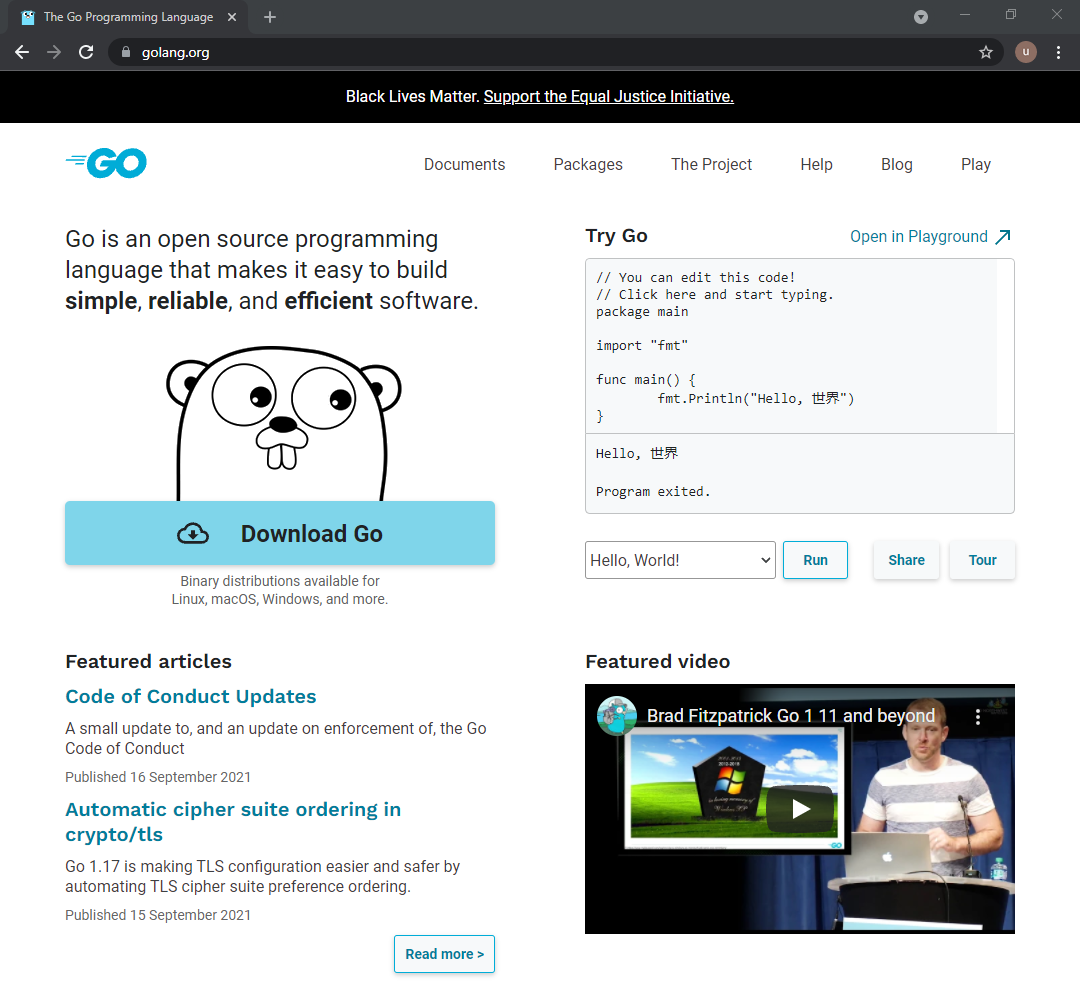
\includegraphics[width=1\linewidth]{00-images/01-download.png}
    \caption{Go programlama dilinin Compiler ını indirebilmek için golang.org sitesinin "Download Go" linkini tıklıyoruz. }
    \label{fig:my_label}
\end{figure}

\vspace{10mm}

\begin{figure}[!htb]
    \centering
    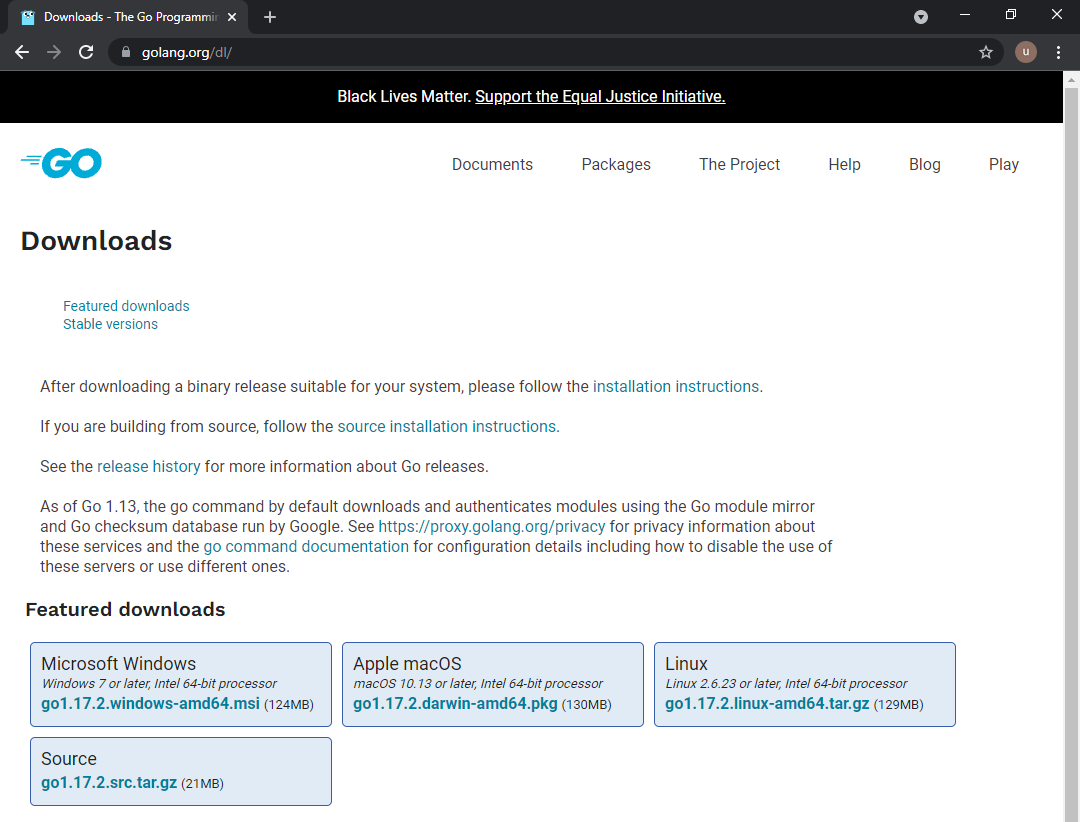
\includegraphics[width=1\linewidth]{00-images/02-download.png}
    \caption{İşletim sistemimize (Windows, macOS, Linux) göre kurulum dosyasını indiriyoruz. }
    \label{fig:my_label}
\end{figure}

\vspace{10mm}

% Installation 1
\begin{figure}[!htb]
    \centering
    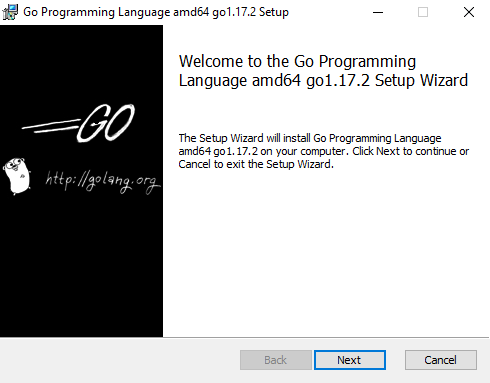
\includegraphics[width=0.6\linewidth]{00-images/03-installation.png}
    \caption{Kurulum dosyasının Next butonuna tıklıyoruz. }
    \label{fig:my_label}
\end{figure}

\vspace{5mm}

% Installation 2
\vspace{10mm}

\begin{figure}[!htb]
    \centering
    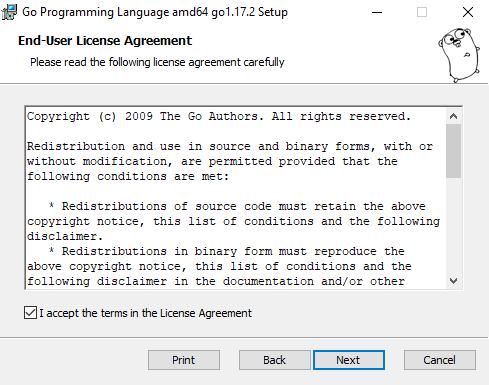
\includegraphics[width=0.6\linewidth]{00-images/04-installation.png}
    \caption{Lisans anlaşmasını kabul edip, Next butonuna tıklıyoruz. }
    \label{fig:my_label}
\end{figure}

\vspace{5mm}

% Installation 3

\begin{figure}[!htb]
    \centering
    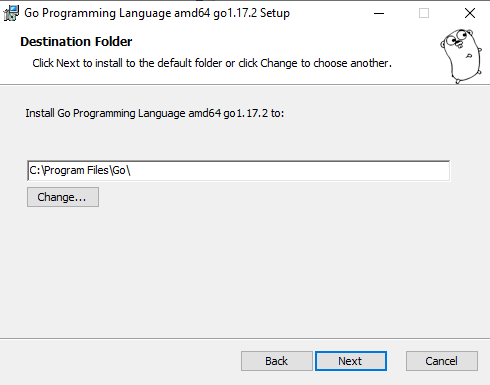
\includegraphics[width=0.6\linewidth]{00-images/05-installation.png}
    \caption{Derleyicinin bilgisayarda hangi alana kurulucağını seçip, Next butonuna tıklıyoruz.}
    \label{fig:my_label}
\end{figure}

\vspace{5mm}

% Installation 4
\vspace{10mm}

\begin{figure}[!htb]
    \centering
    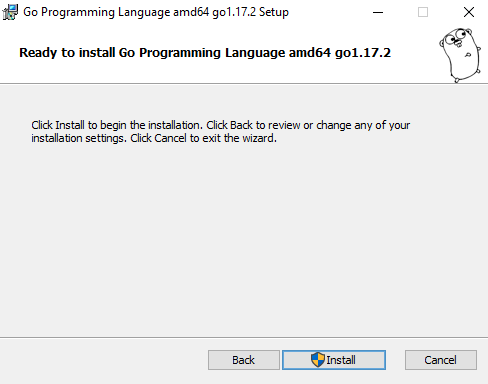
\includegraphics[width=0.6\linewidth]{00-images/06-installation.png}
    \caption{Kurulum için Install butonuna tıklıyoruz.}
    \label{fig:my_label}
\end{figure}

\vspace{5mm}

% Installation 5
\vspace{10mm}

\begin{figure}[!htb]
    \centering
    
\includegraphics[width=0.6\linewidth]{00-images/07-installation.png}
    \caption{Son olarak Finish butonuna tıklıyoruz ve artık Go Dilinin derleyicisi kurulmuş oldu.}
    \label{fig:my_label}
\end{figure}

\vspace{5mm}

% ///////////////////////////////////////////////////////////////////////////
% VERI TIPLERI
% ///////////////////////////////////////////////////////////////////////////

\vspace{15mm}
\section{Veri Tipleri}
\vspace{7mm}

\begin{table}[!htb]
\begin{tabular}{|lcccc|}
\hline
\multicolumn{5}{|c|}{\textbf{Unsigned Integer}}                                                                                                                                                                 \\ \hline
\multicolumn{1}{|l|}{}                          & \multicolumn{1}{c|}{\textbf{uint8}} & \multicolumn{1}{c|}{\textbf{uint16}} & \multicolumn{1}{c|}{\textbf{uint32}} & \textbf{uint64}                           \\ \hline
\multicolumn{1}{|l|}{\textbf{Başlangıç Değeri}} & \multicolumn{1}{l|}{0}              & \multicolumn{1}{l|}{0}               & \multicolumn{1}{l|}{0}               & \multicolumn{1}{l|}{0}                    \\ \hline
\multicolumn{1}{|l|}{\textbf{Bitiş Değeri}}     & \multicolumn{1}{l|}{255}            & \multicolumn{1}{l|}{65535}           & \multicolumn{1}{l|}{4294967295}      & \multicolumn{1}{l|}{18446744073709551615} \\ \hline
\multicolumn{5}{|c|}{\textbf{Integer}}                                                                                                                                                                          \\ \hline
\multicolumn{1}{|l|}{}                          & \multicolumn{1}{c|}{\textbf{int8}}  & \multicolumn{1}{c|}{\textbf{int16}}  & \multicolumn{1}{c|}{\textbf{int32}}  & \textbf{int64}                            \\ \hline
\multicolumn{1}{|l|}{\textbf{Başlangıç Değeri}} & \multicolumn{1}{c|}{-128}           & \multicolumn{1}{c|}{-32768}          & \multicolumn{1}{c|}{-2147483648}     & -9223372036854775808                                         \\ \hline
\multicolumn{1}{|l|}{\textbf{Bitiş Değeri}}     & \multicolumn{1}{c|}{127}            & \multicolumn{1}{c|}{32767}           & \multicolumn{1}{c|}{2147483647}      & 9223372036854775807                                         \\ \hline
\multicolumn{5}{|c|}{\textbf{Float}}                                                                                                                                                                            \\ \hline
\multicolumn{1}{|l|}{}                          & \multicolumn{2}{c|}{\textbf{float32}}                                      & \multicolumn{2}{c|}{\textbf{float64}}                                            \\ \hline
\multicolumn{1}{|l|}{\textbf{Başlangıç Değeri}} & \multicolumn{2}{c|}{-3.4E+38}                                              & \multicolumn{2}{c|}{-1.7E+308}                                                   \\ \hline
\multicolumn{1}{|l|}{\textbf{Bitiş Değeri}}     & \multicolumn{2}{c|}{3.4E+38}                                               & \multicolumn{2}{c|}{1.7E+308}                                                    \\ \hline
\end{tabular}
\end{table}


\vspace{20mm}
\textbf{String Veri Tipi}
\vspace{7mm}

Go dilinde String Veri Tipi karakterleri kelimeleri veya cümleleri tanımlamak için kullanılır ve bunlar tanımlanırken ilk program da verdiğimiz örnekteki gibi "Hello World" çift tırnak içinde tanımlanırlar.

\vspace{5mm}
Go dilinde String Veri Tipi UTF-8 olarak kodlu bir biçimdedir. UTF-8 8 bitlik bir alana sahiptir.


\vspace{20mm}
\textbf{Boolean Veri Tipi}
\vspace{7mm}

Go dilinde Veri Tiplerinin karşılaştırılmasını sağlayan ve bunun sonucunuda "true" doğru ve "false" yanlış olarak geri döndüren veri tipine Boolean Veri Tipi diyoruz.

\vspace{10mm}
Go dilinde İki veri tipini karşılaştırmada $"==", "!=", "<", "<=", ">="$ işaretlerini kullanıyoruz

\vspace{10mm}
Go dilinde $"=="$ işareti iki veri tipinin aynı veri tiplerine sahip olup olmadığını vede aynı değerleri tutup tutmadığını değer olarak "true" yada "false" geri döndürür.

\vspace{10mm}
Go dilinde $"!="$ işareti iki veri tipinin farklı veri tiplerine sahip olup olmadığını vede farklı değerleri tutup tutmadığını değer olarak "true" yada "false" geri döndürür.

\vspace{10mm}
Go dilinde $"<", ">"$ işaretleri bir verinin diğer veri den daha büyük veya daha küçük olup olmadığını ölçer ve bunun sonucunda değer olarak "true" yada "false" geri döndürür.

\vspace{10mm}
Go dilinde $"<=", ">="$  işaretleri bir verinin diğer veri den büyük eşit yada küçük eşit olup olmadığını ölçer ve bunun sonucunda değer olarak "true" yada "false" geri döndürür.
\vspace{10mm}

\lstinputlisting[language=Go]{codes/01-data_types.go}
\captionof{table}{Veri Tipleri}


% ///////////////////////////////////////////////////////////////////////////
% DEGISKEN ATAMA
% ///////////////////////////////////////////////////////////////////////////

\section{Değişken Atama}

\vspace{10mm}

Go dilinde değişken atamaları derleme zamanında statik olarak yapılır. Değişken atama çeşitleri var ve const olarak ikiye ayrılır. 

\vspace{20mm}


\textbf{Variables "var"}
\vspace{10mm}

var ile değişken ataması yaptığımızda atanan değer veri tipi aynı kalmak şartıyla değiştirilebilir.
\vspace{10mm}

\lstinputlisting[language=Go]{codes/02-var_assignment.go}
\captionof{table}{Var Değişken Değer Ataması}


\vspace{20mm}
\textbf{Constants "const"}
\vspace{10mm}

const ile değişken ataması yaptığımızda atanan değer sabit bir şekilde kalır ve değiştirilemez.  
\vspace{5mm}
\lstinputlisting[language=Go]{codes/02-const_assignment.go}
\captionof{table}{Const Sabit Değer Ataması}
\vspace{10mm}

\vspace{10mm}
\textbf{Kısaltılmış Değer Ataması}
\vspace{7mm}

Go dilinde ":=" işareti kullanılarak daha kısa bir şekilde değer ataması mümkündür. 
\vspace{5mm}

\lstinputlisting[language=Go]{codes/02-shorter_assignment.go}
\captionof{table}{Kısaltılmış Değer Ataması}


\vspace{8mm}
\textbf{Çoklu "var" Değer Ataması}
\vspace{7mm}

Go dilinde birden fazla değerin var kullanılarak tek seferde atanması mümkündür.
\vspace{5mm}

\lstinputlisting[language=Go]{codes/02-multiple_variable_assingment.go}
\captionof{table}{Birden Fazla Değişken Değer Ataması}

\vspace{10mm}
\textbf{Çoklu "const" Değer Ataması}
\vspace{7mm}

Go dilinde birden fazla değerin const kullanılarak tek seferde atanması mümkündür.
\vspace{5mm}
\lstinputlisting[language=Go]{codes/02-multiple_constant_assingment.go}
\captionof{table}{Birden Fazla Sabit Değer Ataması}


\vspace{20mm}
\textbf{Global Scope Değer Ataması}
\vspace{7mm}

Go dilinde fonksiyon dışlarında global değer atamaları yapılabilir ve bu atanan değerlere fonksiyonlardan erişim sağlanabilir.
\vspace{10mm}
\lstinputlisting[language=Go]{codes/02-global_scope.go}
\captionof{table}{Global Scope Değer Ataması}


\vspace{10mm}
\textbf{Local Scope Değer Ataması}
\vspace{5mm}

Go dilinde fonksiyon içlerinde local değer atamaları yapılabilir ve bu atanan değerlere direkt olarak ancak fonksiyon içerisinden erişim sağlanabilir.
\vspace{5mm}

\lstinputlisting[language=Go]{codes/02-local_scope.go}
\captionof{table}{Local Scope Değer Ataması}

% ///////////////////////////////////////////////////////////////////////////
% KONTROL YAPILARI
% ///////////////////////////////////////////////////////////////////////////

\section{Kontrol Yapilari}
\vspace{5mm}

Go dilinde complex problemlerle karşılaşabiliriz bunların çözümünde "for, if, switch" gibi kontrol yapılarını kullanabiliriz. 

\vspace{20mm}


\textbf{Döngüler "for"}
\vspace{7mm}

for ile değişkenlerimizi döngüde tutarak istediğimiz işlemleri birden fazla işlem basamağıyla gerçekleştirebiliriz.
\vspace{5mm}
\lstinputlisting[language=Go]{codes/05-for_loop.go}
\captionof{table}{For Döngüsü}


\vspace{10mm}
\textbf{Döngüler "while"}
\vspace{5mm}

Go dilinde diğer dillerde olduğu gibi ayrı bir "while" döngü yapısı kullanılmak yerine for döngüsü ile while döngüsünü oluşturabiliyoruz.
\vspace{5mm}
\lstinputlisting[language=Go]{codes/05-while_loop.go}
\captionof{table}{While Döngüsü}


\vspace{10mm}
\textbf{Karar Yapısı "if,else if, else"}
\vspace{5mm}

if, else if, else ile değişkenlerimizin doğruluk sağlayıp sağlamamasına göre işlem karar mekanizmaları oluşturabiliriz.
\vspace{5mm}

\lstinputlisting[language=Go]{codes/05-if_else.go}
\captionof{table}{If, Else Yapıları}

\vspace{10mm}
\textbf{Karar Yapısı "switch case"}
\vspace{5mm}

switch case ile değişkenlerimizin doğruluk sağlayıp sağlamamasına göre işlem karar mekanizmaları oluşturabiliriz.
\vspace{5mm}
\lstinputlisting[language=Go]{codes/05-switch_case.go}
\captionof{table}{Switch Case Yapısı}

% ///////////////////////////////////////////////////////////////////////////
% ARRAYS, SLICES, MAPS
% ///////////////////////////////////////////////////////////////////////////

\section{Arrays, Slices, Maps}
\vspace{5mm}

Go dilinde verileri gruplandırmak ve bir arada tutmak için "arrays, slices, maps" gibi veri yapılarını kullanıyoruz. 
\vspace{10mm}

\textbf{Diziler "arrays"}
\vspace{5mm}

Go dilinde sabit uzunluklu diziler tanımlayabiliriz.
\vspace{5mm}

\lstinputlisting[language=Go]{codes/06-fixed_size_array.go}
\captionof{table}{Sabit Uzunlukdaki Diziler}


\vspace{10mm}
\textbf{Slices}
\vspace{5mm}

Go dilinde dizilerin uzerine inşa edilmiş slice yapısı bulunmaktadır. Bu yapılar dinamik olarak uzunluğunu arttırabilir yada azaltabilir.
\vspace{5mm}

\lstinputlisting[language=Go]{codes/06-slices.go}
\captionof{table}{Slices}

\vspace{20mm}
\textbf{Ekleme "append"} append ile dizilerimize veri ekleyebiliyoruz.
\vspace{5mm}
\lstinputlisting[language=Go]{codes/06-append.go}
\captionof{table}{Diziye Veri Ekleme}


\vspace{10mm}
\textbf{Çok Boyutlu Diziler}
\vspace{5mm}

Multi Dimensional Arrays ile çok boyutlu veri dizileri oluşturabiliyoruz.
\vspace{5mm}
\lstinputlisting[language=Go]{codes/06-multi_dimensional.go}
\captionof{table}{Çok Boyutlu Diziler}


\vspace{20mm}
\textbf{Maps}
\vspace{5mm}

Maps ile anahtar değer ilişkisiyle veri tutabilen veri yapısıdır. Bilgisayar bilimlerinde genel olarak Hash Table olarak bilinir
\vspace{5mm}
\lstinputlisting[language=Go]{codes/06-map.go}
\captionof{table}{Map}


\vspace{10mm}
\textbf{Append, Delete}
\vspace{5mm}

Maps de veri eklemeyi yeni bir anahtar değer ekliyerek vede silmek için ise Delete fonksiyonunu kullanıyoruz.
\vspace{5mm}
\lstinputlisting[language=Go]{codes/06-map_append_delete.go}
\captionof{table}{Map Ekleme ve Silme}

% ///////////////////////////////////////////////////////////////////////////
% FONKSIYONLAR
\newpage
% ///////////////////////////////////////////////////////////////////////////

\section{Fonksiyonlar}

\vspace{10mm}

Go dilinde "functions" olarak adlandırılan kod blokları bulunmaktadır. Fonksiyonlar genel olarak karmaşık problemlerin çözümünde modülerlik açısından karmaşıklığın azaltılması ve kodun tekrar kullanılabilirliğinin arttırılması için kullanılır.
\vspace{5mm}

Bu kod blokları birden fazla parametre alabiliceği gibi hiç parametre almayadabilir. Aynı şekilde birden fazla değer geri döndürebiliceği gibi hiç geri değer döndürmeyedebilir.

\vspace{20mm}


\textbf{Fonksiyonlar}
\vspace{5mm}

Go dilinde şu ana kadar sadece Main Fonksiyonunu kullanıyorduk. 
\vspace{5mm}
\lstinputlisting[language=Go]{codes/07-main_function.go}
\captionof{table}{Main Function}

\vspace{10mm}
\textbf{Değer Almayan ve Döndürmeyen Fonksiyonlar}
\vspace{5mm}

Go dilinde fonksiyonların herhangi bir değer alması veya döndürmesi zorunlu değildir.
\vspace{5mm}
\lstinputlisting[language=Go]{codes/07-dummy_func.go}
\captionof{table}{Dummy Function}


\vspace{10mm}
\textbf{Değer Alan Fonksiyonlar}
\vspace{5mm}

Go dilinde bir veya birden fazla değer alan fonksiyonlar yazılabilir.
\vspace{5mm}
\lstinputlisting[language=Go]{codes/07-func_args.go}
\captionof{table}{Fonksiyon Argumanları}


\vspace{10mm}
\textbf{Değer Döndüren Fonksiyonlar}
\vspace{5mm}

Değer döndüren fonksiyonlarda fonksiyon ismi tanımlandıktan sonra döndürülücek değer tipleri tanımlaması yapılır.
\vspace{5mm}
\lstinputlisting[language=Go]{codes/07-return_value.go}
\captionof{table}{Değer Döndüren Fonksiyonlar}

\vspace{20mm}
\textbf{Birden Fazla Değer Alan ve Birden Fazla Değer Döndüren Fonksiyonlar}
\vspace{5mm}

Go dilinde fonksiyonlar birden fazla değer alabildiği gibi birden fazla değer döndürebilirler.
\vspace{5mm}


\lstinputlisting[language=Go]{codes/07-multiple_args_returns.go}
\captionof{table}{Birden Fazla Değer Alan ve Birden Fazla Değer Döndüren Fonksiyonlar}


\vspace{10mm}
\textbf{Defer, Panic ve Recover}
\vspace{5mm}

\textbf{Defer} kullandığımız fonksiyon çağırıldığı fonksiyon bloğunun bitmesini bekler ve ardından çalışır.
\vspace{5mm}
\lstinputlisting[language=Go]{codes/07-defer.go}
\captionof{table}{Defer}

\vspace{10mm}
\textbf{Panic} çalışma zamanı hatasına sebep olur.
\vspace{5mm}
\lstinputlisting[language=Go]{codes/07-panic.go}
\captionof{table}{Panic}

\vspace{10mm}
\textbf{Recover} panic kullanarak sebep olduğumuz çalışma zamanı hatasından defer ve recover fonksiyonlarıni kullanarak kurtuluruz.
\vspace{5mm}
\lstinputlisting[language=Go]{codes/07-recover.go}
\captionof{table}{Recover}

% ///////////////////////////////////////////////////////////////////////////
% POINTERS
% ///////////////////////////////////////////////////////////////////////////
\section{Pointers}
\vspace{5mm}

Go dilinde "pointer" referansları bulunmaktadır ve bu referanslar kullandığımız değerin bellekteki adresini temsil eder.
\vspace{20mm}

\textbf{\& Referans Operatörü } 
\vspace{7mm}

\& operatörü oluşturduğumuz değerlerin bellek adreslerine ulaşmamızı sağlar.

\vspace{5mm}
\lstinputlisting[language=Go]{codes/08-and_operator.go}
\captionof{table}{\& Operatörü}

\vspace{10mm}

\textbf{* Referans Operatörü } 
\vspace{7mm}

* operatörü adres referans bilgisine sahip olduğumuz değerleri bize verir.

\vspace{5mm}
\lstinputlisting[language=Go]{codes/08-multiply_operator.go}
\captionof{table}{\* Operatörü}


\vspace{10mm}
\textbf{Referans Örneği}
\vspace{5mm}

Aşağıdaki örnekde adres değeri kullanılarak değişken değeri değiştirilmiştir.

\vspace{5mm}
\lstinputlisting[language=Go]{codes/08-pointer_example.go}
\captionof{table}{Pointer Örneği}

\vspace{10mm}

% ///////////////////////////////////////////////////////////////////////////
% STRUCT VE INTERFACE
\newpage
% ///////////////////////////////////////////////////////////////////////////

\section{Struct ve Interface}
\vspace{5mm}

Struct Go Dilinde Verilerin Düzenli Bir Şekilde Tutulması İçin Kullanılır.
\vspace{7mm}


\vspace{5mm}
\lstinputlisting[language=Go]{codes/09-struct.go}
\captionof{table}{Struct}

\vspace{10mm}

\textbf{Struct Örneği}
\vspace{10mm}

Aşağıdaki örnekde struct direk olarak değişken tipleri belirtilmiş ve bir değişkene atanmıştır.

\vspace{10mm}
\lstinputlisting[language=Go]{codes/09-struct_example.go}
\captionof{table}{Struct Örneği}

\vspace{10mm}

Interface Go Dilinde bir veya daha fazla Methodun Method İmzaları kullanılarak bir arada toplanması için kullanılan bir yapıdır.
\vspace{10mm}

\lstinputlisting[language=Go]{codes/09-interface.go}
\captionof{table}{Interface}

\vspace{10mm}

\textbf{Interface Örneği} 
\vspace{5mm}

Aşağıdaki interface örneğinde kare ve dairenin alanı struct olarak tanımlandı ve method imzaları olan 'square' and 'circle' method koleksiyonu olan 'shape' üzerinde tanımlaması yapıldı.

\lstinputlisting[language=Go]{codes/09-interface_example.go}
\captionof{table}{Interface Örneği}

\vspace{10mm}

% ///////////////////////////////////////////////////////////////////////////
% CONCURRENCY
% ///////////////////////////////////////////////////////////////////////////

\section{Concurrency}
\vspace{5mm}

Goroutines Go dilinde threadlerin yerine kullanabiliceğimiz daha az kaynak tüketimi olan goroutine(sanal thread) ler bulunmaktadır. Her bir programın içerisinde en az bir goroutine bulunmaktadır ve bu goroutine 'main goroutine' olarak adlandırılır.Diğer bütün goroutineler 'main goroutine' in altında çalışırlar.

\vspace{5mm}
\lstinputlisting[language=Go]{codes/10-goroutines.go}
\captionof{table}{Goroutines}

\vspace{10mm}

\textbf{Goroutines Örnek}
\vspace{10mm}

Aşağıdaki örnekde multithreading i simüle edebilmek için 'time.Sleep' fonksiyonundan yararlanılmıştır fakat bu fonksiyonun kaynak tüketimi yüksektir bu yüzden kaynak tüketimi daha az olan  'sync.WaitGroup' fonksiyonlarını kullanacağız.

\vspace{10mm}

\lstinputlisting[language=Go]{codes/10-goroutines_example_1.go}
\captionof{table}{Goroutine Örneği}

\vspace{10mm}

\textbf{Goroutines Örnek 2}
\vspace{10mm}

Aşağıdaki örnekde 'time.Sleep' fonksiyonu yerine  'sync.WaitGroup' fonksiyonları kullanıldı.

\vspace{10mm}
\lstinputlisting[language=Go]{codes/10-goroutines_example_2.go}
\captionof{table}{Goroutine Örneği 2}
\vspace{10mm}

\textbf{Channels}
\vspace{5mm}

Channels, eşzamanlı goroutinleri birbirine bağlayan kanallardır. Bir goroutinden Channels üzerinden değerler gönderebilir ve bu değerleri başka bir goroutine ile Channels üzerinden alabilirsiniz.
\vspace{10mm}

\lstinputlisting[language=Go]{codes/10-channels.go}
\captionof{table}{Channels}

\vspace{10mm}

\textbf{Channels Örnek}

\vspace{10mm}
\lstinputlisting[language=Go]{codes/10-channels_example.go}
\caption{Channels Örneği}

\vspace{10mm}

% ///////////////////////////////////////////////////////////////////////////

% \centering
% /////////////////////////////////////////////////////////////////////
\chapter{Soket Programlama}

%----------------------------
\vspace{10mm}
\section{Giriş}
Soketler, aynı veya farklı makinelerdeki iki farklı işlem arasında iletişime izin verir. Daha kesin olmak gerekirse, standart Unix dosya tanımlayıcılarını kullanarak diğer bilgisayarlarla konuşmanın bir yolu. Unix'te her G/Ç eylemi, bir dosya tanıtıcısı yazılarak veya okunarak yapılır. Dosya tanımlayıcı yalnızca açık bir dosyayla ilişkili bir tamsayıdır ve bir ağ bağlantısı, metin dosyası, terminal veya başka bir şey olabilir.


\vspace{10mm}

\section{Soket Programlama Uygulama Alanları}

Bir istemci-sunucu uygulama çerçevesinde bir Unix Soketi kullanılır. Sunucu, bir istemciden gelen istek üzerine bazı işlevleri yerine getiren bir işlemdir. FTP, SMTP ve POP3 gibi uygulama düzeyindeki protokollerin çoğu, istemci ve sunucu arasında bağlantı kurmak ve ardından veri alışverişi için soketleri kullanır.
Soket Programlama TCP kullanarak istemci ve sunucu arasında bir bağlantı oluşturuyoruz, TCP yüksek güvenilirlik gerektiren uygulamalar için uygundur ve iletim süresi nispeten daha az kritiktir. HTTP, HTTPs, FTP, SMTP, Telnet gibi diğer protokoller tarafından kullanılır. TCP, veri paketlerini belirtilen sırada yeniden düzenler. Aktarılan verilerin bozulmadan kaldığına ve gönderildiği sırayla ulaştığına dair mutlak bir garanti vardır. TCP, Akış Kontrolü yapar ve herhangi bir kullanıcı verisi gönderilmeden önce bir soket bağlantısı kurmak için üç paket gerektirir. TCP, güvenilirlik ve tıkanıklık kontrolünü ele alır. Ayrıca hata denetimi ve hata kurtarma da yapar. Hatalı paketler kaynaktan hedefe yeniden iletilir.
\vspace{10mm}

% ///////////////////////////////////////////////////////////////////
\newpage
\section{OSI Katmanları}
\begin{figure}[!htb]
    \centering
    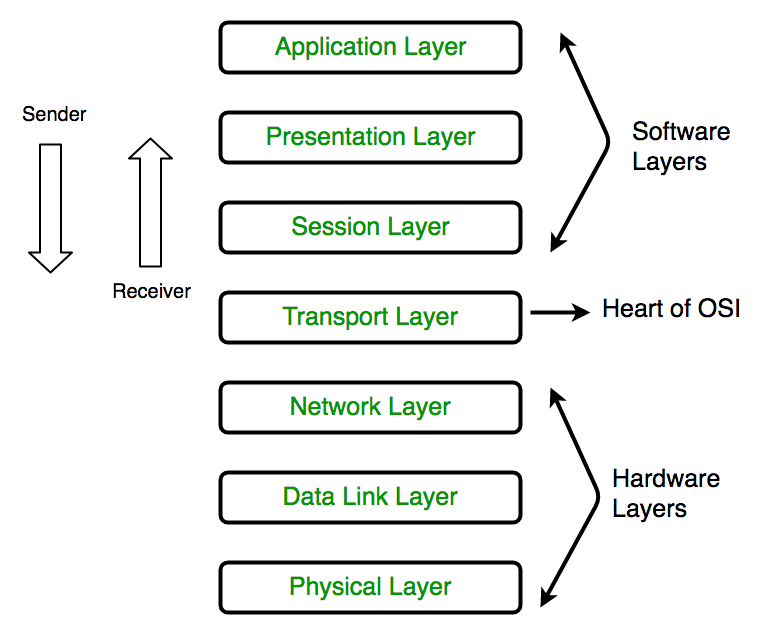
\includegraphics[width=1\linewidth]{00-images/08-osi_layers.png}
    \caption{OSI Katmanları}
    \label{fig:my_label}
\end{figure}


\vspace{10mm}
\textbf{1. Fiziksel Katman}
\vspace{5mm}

Fiziksel katman, ağ düğümleri arasındaki fiziksel kablo veya kablosuz bağlantıdan sorumludur. Cihazları bağlayan konektörü, elektrik kablosunu veya kablosuz teknolojiyi tanımlar ve bit hızı kontrolü ile ilgilenirken, sadece bir dizi 0 ve 1 olan ham verilerin iletilmesinden sorumludur.

\vspace{10mm}
\textbf{2. Veri Bağlantı Katmanı}
\vspace{5mm}

Veri bağlantı katmanı, bir ağ üzerinde fiziksel olarak bağlı iki düğüm arasında bir bağlantı kurar ve sonlandırır. Paketleri çerçevelere böler ve kaynaktan hedefe gönderir. Bu katman iki bölümden oluşur: Ağ protokollerini tanımlayan, hata denetimi gerçekleştiren ve çerçeveleri senkronize eden Mantıksal Bağlantı Kontrolü (LLC) ve cihazları bağlamak ve veri iletmek ve almak için izinleri tanımlamak için MAC adreslerini kullanan Medya Erişim Kontrolü (MAC).

\vspace{10mm}
\textbf{3. Ağ Katmanı}
\vspace{5mm}

Ağ katmanının iki ana işlevi vardır. Biri, segmentleri ağ paketlerine bölmek ve paketleri alıcı uçta yeniden birleştirmek. Diğeri ise paketleri fiziksel bir ağ üzerinde en iyi yolu keşfederek yönlendirmektir. Ağ katmanı, paketleri bir hedef düğüme yönlendirmek için ağ adreslerini (tipik olarak İnternet Protokolü adresleri) kullanır.

\vspace{10mm}
\textbf{4. Taşıma Katmanı}
\vspace{5mm}

Taşıma katmanı, oturum katmanında aktarılan verileri alır ve iletim tarafında “bölümlere” ayırır. Alıcı taraftaki segmentleri yeniden birleştirmek ve oturum katmanı tarafından kullanılabilecek verilere dönüştürmekten sorumludur. Taşıma katmanı, akış kontrolünü, alıcı cihazın bağlantı hızına uygun bir hızda veri gönderme ve hata kontrolünü, verinin yanlış alınıp alınmadığını kontrol edip, değilse tekrar talep ederek gerçekleştirir.

\vspace{10mm}
\textbf{5. Oturum Katmanı}
\vspace{5mm}

Oturum katmanı, cihazlar arasında oturum adı verilen iletişim kanalları oluşturur. Oturumların açılmasından, veriler aktarılırken açık ve işlevsel kalmasının sağlanmasından ve iletişim sona erdiğinde kapatılmasından sorumludur. Oturum katmanı ayrıca veri aktarımı sırasında kontrol noktaları ayarlayabilir; oturum kesilirse cihazlar son kontrol noktasından veri aktarımına devam edebilir.

\vspace{10mm}
\textbf{6. Sunum Katmanı}
\vspace{5mm}

Sunum katmanı, uygulama katmanı için verileri hazırlar. Diğer uçta doğru şekilde alınması için iki cihazın verileri nasıl kodlaması, şifrelemesi ve sıkıştırması gerektiğini tanımlar. Sunum katmanı, uygulama katmanı tarafından iletilen herhangi bir veriyi alır ve oturum katmanı üzerinden aktarım için hazırlar.

\vspace{10mm}
\textbf{7. Uygulama Katmanı}
\vspace{5mm}

Uygulama katmanı, web tarayıcıları ve e-posta istemcileri gibi son kullanıcı yazılımları tarafından kullanılır. Yazılımın bilgi gönderip almasına ve kullanıcılara anlamlı veriler sunmasına izin veren protokoller sağlar. Uygulama katmanı protokollerine birkaç örnek, Hypertext Transfer Protocol (HTTP), File Transfer Protocol (FTP), Post Office Protocol (POP), Simple Mail Transfer Protocol (SMTP), Domain Name System (DNS).

% ///////////////////////////////////////////////////////////////////

\vspace{20mm}
\section{TCP/UDP Protokolleri}
\begin{figure}[!htb]
    \centering
    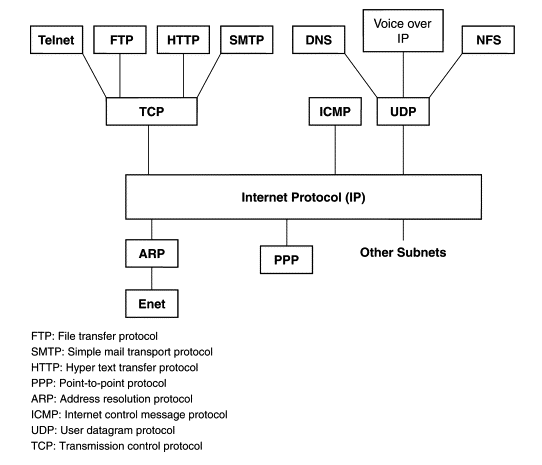
\includegraphics[width=1\linewidth]{00-images/11-network.png}
    \caption{TCP/UDP Protokolleri}
    \label{fig:my_label}
\end{figure}

\vspace{10mm}
\textbf{İnternet Protokolü}
\vspace{5mm}

Genel olarak konuşmak gerekirse internet birbirine bağlanan cihazlar bütünüdür. Akıllı telefonunuz, kişisel bilgisayarınız veya sunucunuz olsun, her cihaz internet protokol paketi aracılığıyla iletişim kurar. İnternet protokol paketi, cihazların birbirleriyle iletişim kurması için farklı protokoller veya yöntemler topluluğudur. Hem TCP hem de UDP, internet protokol paketindeki ana protokollerdir. İnternete bağlı her cihazın benzersiz bir IP adresi vardır. Herhangi iki cihaz internet protokolü üzerinden iletişim kurmak isterse TCP veya UDP protokolünü kullanır.

\begin{figure}[!htb]
    \centering
    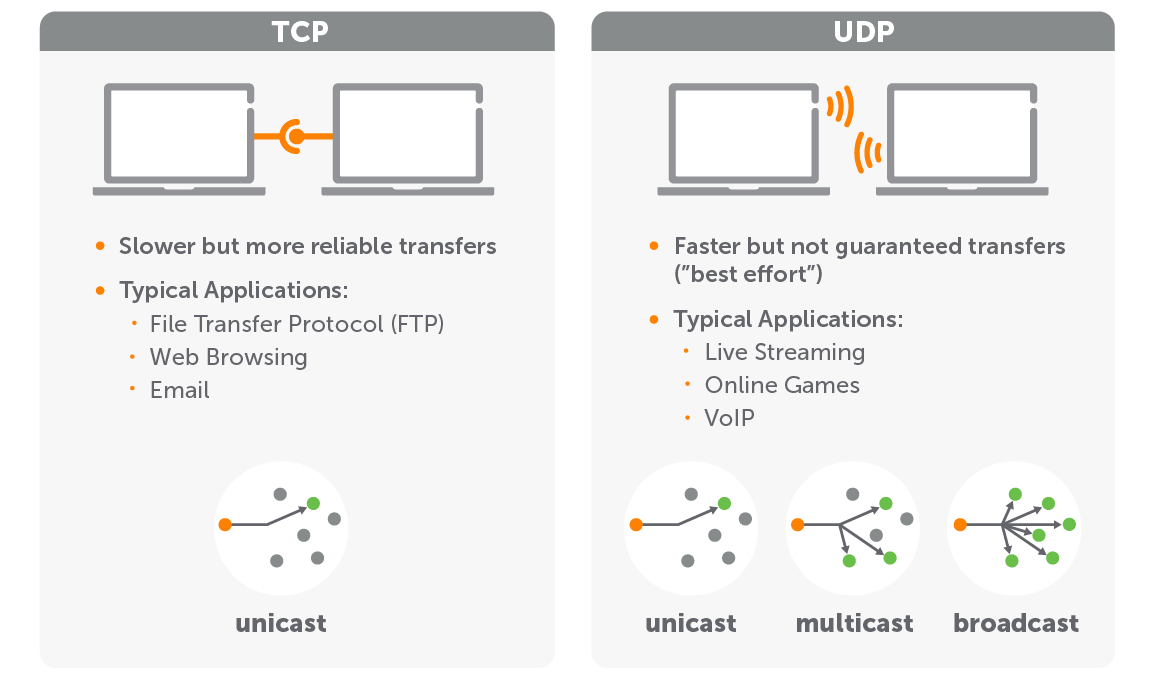
\includegraphics[width=1\linewidth]{00-images/12-tcp_udp.png}
    \caption{TCP/UDP Protokol Karşılaştırılması}
    \label{fig:my_label}
\end{figure}

\vspace{10mm}
\textbf{TCP Protokolü}
\vspace{5mm}

TCP veya İletim Kontrol Protokolü (Transmission Control Protocol), çevrimiçi olarak en yaygın ağ protokolüdür. TCP son derece güvenilirdir ve internette gezinmeye (HTTP), e-posta göndermeye (SMTP) ve dosya aktarmaya (FTP) kadar her şey için kullanılır.
TCP, bir cihaz tarafından gönderilen tüm verilerin başka bir cihaz tarafından tamamen bozulmamış olarak alınmasının gerekli olduğu durumlarda kullanılır.
Örneğin, bir web sitesini ziyaret ettiğinizde, sayfayı oluşturmak için gereken metin, resim ve koddaki her şeyin size ulaştığını garanti etmek için TCP kullanılır. TCP olmadan, resimler veya metinler eksik olabilir veya yanlış sırada gelerek sayfayı bozabilir.
TCP, bağlantı yönelimli bir protokoldür, yani veri aktarmadan önce iki cihaz arasında bir bağlantı kurar ve aktarım işlemi boyunca bu bağlantıyı korur.
TCP, iki cihaz arasında bağlantı kurmak için üç yönlü handshake adı verilen bir yöntem kullanır.


\begin{figure}[!htb]
    \centering
    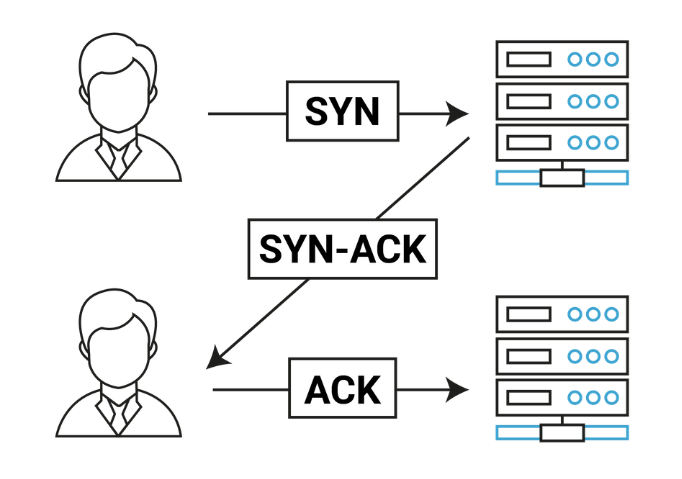
\includegraphics[width=1\linewidth]{00-images/13-tcp.png}
    \caption{Üç Yönlü Handshake}
    \label{fig:my_label}
\end{figure}

\vspace{10mm}
\textbf{Üç Yönlü Handshake}
\vspace{5mm}

Örneğin, cihazınızda bir haber okumak için cihazınız önce SYN (Senkronizasyon Sıra Numarası) adlı o Haber Sitesinin Sunucusuna bir mesaj gönderir. 
Ardından Haber Sitesinin Sunucusu, SYN-ACK adı verilen bir onay mesajını geri gönderir.
Cihazınız sunucudan SYN-ACK aldığında, bağlantıyı kuran bir ACK onay mesajı gönderir.
İki cihaz arasında bir TCP bağlantısı kurulduğunda, protokol tüm verilerin iletilmesini garanti eder.
Cihazınız ve Haber Sitesi örneğine geri dönersek, üç yönlü anlaşma tamamlandıktan sonra Haber Sitesinin Sunucusu, cihazınızın web tarayıcısının makaleyi oluşturmak için ihtiyaç duyduğu tüm verileri göndermeye başlayabilir.
Tüm cihazlar, verileri internet üzerinden göndermeden önce küçük paketlere ayırır. Bu paketlerin daha sonra diğer uçta yeniden birleştirilmesi gerekir.
Bu nedenle, Haber Sitesinin Sunucusu bu makale için HTML, CSS, Resimler ve diğer Kodları gönderdiğinde, bunları cihazınıza göndermeden önce her şeyi küçük veri paketlerine böler. Cihazınız daha sonra bu paketleri, bu makaleyi oluşturmak için ihtiyaç duyduğu dosyalara ve görüntülere yeniden birleştirir.
TCP, bu paketlerin tümünün cihazınıza ulaşmasını sağlar. Yol boyunca herhangi bir paket kaybolursa, TCP, cihazınızın sunucunun eksik veri olduğunu bilmesini ve sunucunun bu paketleri yeniden göndermesini kolaylaştırır.
Cihazınız makaleyi oluşturmak için ihtiyaç duyduğu tüm verileri aldığında, TCP, bu sefer FIN ve ACK paketlerini kullanarak üç yönlü Handshake benzer bir yöntemle iki cihaz arasındaki bağlantıyı otomatik olarak sonlandırır.

\vspace{15mm}

\begin{figure}[!htb]
    \centering
    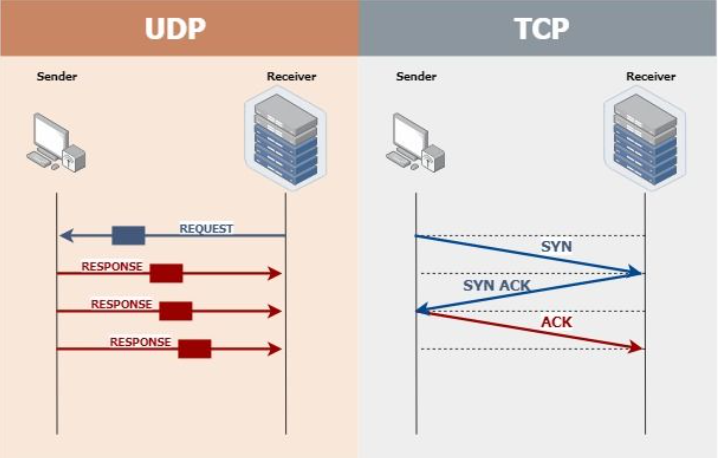
\includegraphics[width=1\linewidth]{00-images/14-tcp_udp.png}
    \caption{TCP/UDP Protokol Farkları}
    \label{fig:my_label}
\end{figure}


\vspace{10mm}
\textbf{UDP Protokolü}
\vspace{5mm}

UDP veya Kullanıcı Datagram Protokolü (User Datagram Protocol), internet protokol paketini oluşturan ana protokollerden bir diğeridir. UDP, TCP'den daha az güvenilirdir, ancak çok daha basittir.
UDP, canlı video/ses gibi bazı veri kayıplarının kabul edilebilir olduğu veya çevrimiçi oyunlar gibi hızın kritik bir faktör olduğu durumlarda kullanılır.
UDP, çevrimiçi veri göndermek ve almak için kullanıldığı için TCP'ye benzer olsa da, birkaç önemli fark vardır.
Birincisi, UDP bağlantısız bir protokoldür, yani TCP'nin üç yönlü handshake ile yaptığı gibi önceden bir bağlantı kurmaz.
Ardından, UDP tüm verilerin başarıyla aktarıldığını garanti etmez. UDP ile, dinlemeye başlayan herhangi bir cihaza veri gönderilir, ancak bir kısmının yolda kaybolması umurunda değildir. UDP'nin "ateşle ve unut" (fire and forget) protokolü olarak da bilinmesinin nedenlerinden biri de budur.
Bu farklılıklar hakkında düşünmenin iyi bir yolu, TCP'nin iki kişi arasındaki bir konuşma gibi olmasıdır. A kişisi B kişisinden konuşmasını ister. B kişisi kabul eder ve ikisi de konuşmaya başlar.
UDP daha çok dışarıda megafonlu bir satıcıya benzer. Satıcıya dikkat eden herkes, söylediklerinin çoğunu duyabilir. Ancak bölgedeki herkesin Satıcının söylediklerini duyacağının veya hatta dinlediklerinin garantisi yoktur.

\vspace{10mm}

% ///////////////////////////////////////////////////////////////////

\section{İnternet Protokolü ve Portlar}

\vspace{5mm}
\textbf{İnternet Protokolü}
\vspace{5mm}

İnternet Protokolü (IP), ağlar arasında transfer edilebilmeleri ve doğru hedefe varabilmeleri için veri paketlerini yönlendirmek ve adreslemek için bir protokol veya kurallar dizisidir. İnternette dolaşan veriler, paket adı verilen daha küçük parçalara bölünür. Her pakete IP bilgisi eklenir ve bu bilgi yönlendiricilerin paketleri doğru yere göndermesine yardımcı olur. İnternete bağlanan her cihaza veya etki alanına bir IP adresi atanır ve paketler bunlara bağlı IP adresine yönlendirildikçe veriler ihtiyaç duyulan yere ulaşır. Paketler hedeflerine ulaştığında, IP ile birlikte hangi taşıma protokolünün kullanıldığına bağlı olarak farklı şekilde işlenirler. En yaygın aktarım protokolleri TCP ve UDP'dir.

\vspace{10mm}
\textbf{İnternet Protokol Versiyon 4}
\vspace{5mm}

İnternet Protokolü Versiyon 4 (IPv4), İnternet Protokolünün (IP) dördüncü sürümüdür. İnternette ve diğer paket anahtarlamalı ağlarda standartlara dayalı ağlar arası çalışma yöntemlerinin temel protokollerinden biridir. IPv4, 1982'de SATNET'te ve Ocak 1983'te ARPANET'te üretim için dağıtılan ilk sürümdü. Bugün hala çoğu İnternet trafiğini yönlendirmek için kullanılıyor.
IPv4, 4,294,967,296 $(2^{32})$ benzersiz adres sağlayan 32 bitlik bir adres alanı kullanır, ancak büyük bloklar özel ağ oluşturma amaçları için ayrılmıştır.

\begin{figure}[!htb]
    \centering
    
\includegraphics[width=1\linewidth]{00-images/10-internet_protocol_v4.png}
    \caption{Internet Protokol Versiyon 4}
    \label{fig:my_label}
\end{figure}

\vspace{10mm}
\textbf{İnternet Protokol Versiyon 6}
\vspace{5mm}

İnternet Protokolü sürüm 6 (IPv6), ağlardaki bilgisayarlar için bir tanımlama ve konum sistemi sağlayan ve trafiği İnternet üzerinden yönlendiren iletişim protokolü olan İnternet Protokolü'nün (IP) en son sürümüdür. IPv6, Internet Engineering Task Force (IETF) tarafından uzun zamandır beklenen IPv4 adres tükenmesi sorunuyla başa çıkmak için geliştirildi ve IPv4'ün yerini alması amaçlandı. Aralık 1998'de IPv6, IETF için Taslak Standart oldu ve daha sonra 14 Temmuz 2017'de bir İnternet Standardı olarak onaylandı. IPv6, 340,282,366,920,938,463,463,374,607,431,768,211,456 $(2^{128})$ benzersiz adres sağlayan 128 bitlik bir adres alanı kullanır.

\begin{figure}[!htb]
    \centering
    
\includegraphics[width=1\linewidth]{00-images/10-internet_protocol_v6.png}
    \caption{Internet Protokol Versiyon 6}
    \label{fig:my_label}
\end{figure}

\newpage

\vspace{10mm}
\textbf{IPv4 ve IPv6 Karşılaştırılması}
\vspace{5mm}

\begin{figure}[!htb]
    \centering
    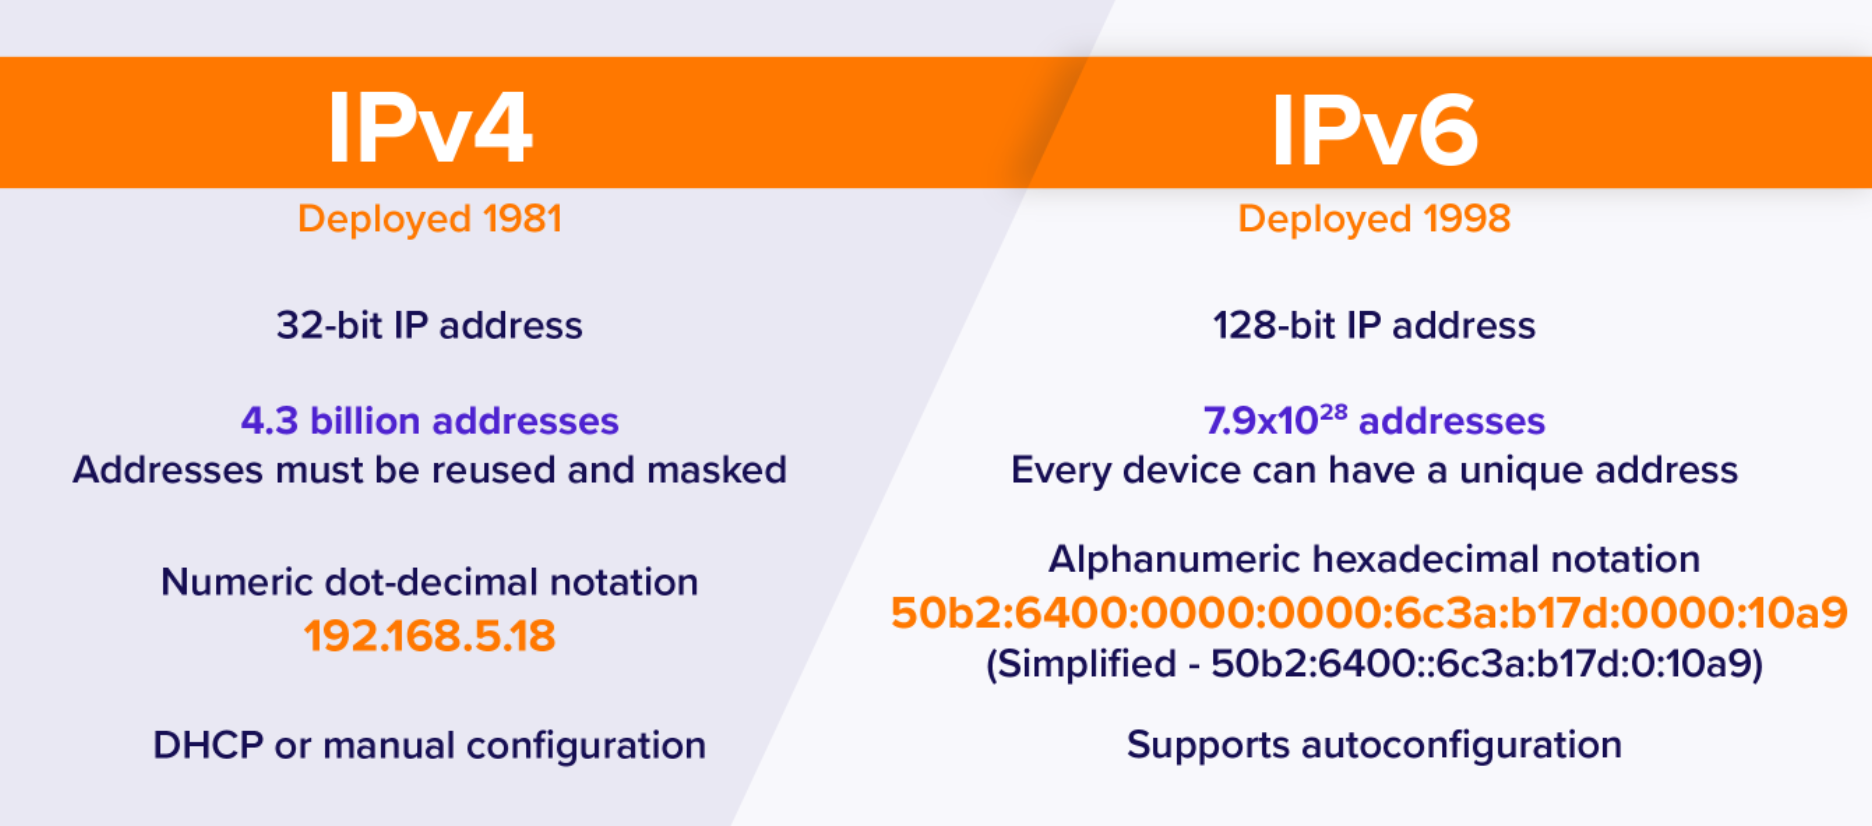
\includegraphics[width=1\linewidth]{00-images/15-ipv4_vs_ipv6.png}
    \caption{IPv4 ve IPv6 Karşılaştırılması}
    \label{fig:my_label}
\end{figure}

\begin{figure}[!htb]
    %
    \centering
    \subfloat[\centering IPv4 Header]{{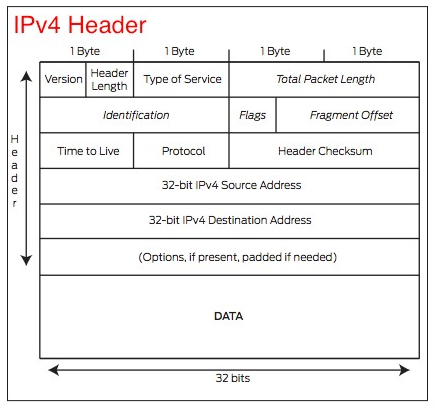
\includegraphics[width=6.6cm]{00-images/15-ipv4_header.png} }}%
    \qquad
    \subfloat[\centering IPv6 Header]{{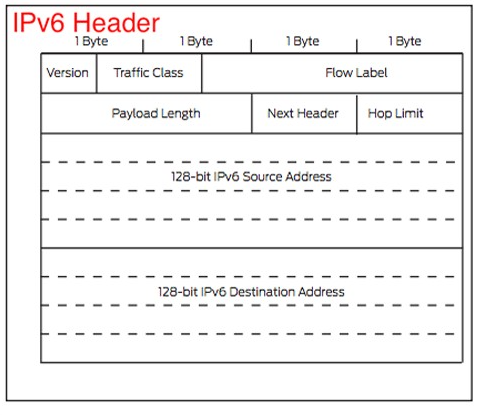
\includegraphics[width=7cm]{00-images/15-ipv6_header.png} }}%
    \caption{IPv4 ve IPv6 Header Karşılaştırılması}%
    \label{fig:example}
    %
\end{figure}



\newpage

\vspace{10mm}
\textbf{Portlar}
\vspace{5mm}

Port numarası, bilgisayar ağlarında mesajların göndericilerini ve alıcılarını tanımlamak için kullanılan adresleme bilgilerinin bir parçasıdır. Gelen trafiğin hangi protokole yönlendirileceğini belirlemek için farklı port numaraları kullanılır. Bağlantı noktası numarası, bir İnternet veya başka bir ağ mesajının bir sunucuya ulaştığında iletileceği belirli bir işlemi tanımlar. Her protokol için bağlantı noktaları tanımlanır ve bir iletişim uç noktası olarak kabul edilir.

Bağlantı noktaları 16 bitlik sayılarla temsil edilir. 65336  $(2^{16})$ bağlantı noktası numarası vardır.

\vspace{10mm}
\textbf{Port Grupları}
\vspace{5mm}

0 ila 1023 - İyi bilinen (Well Known) port numaraları. Yalnızca Apple QuickTime, MSN, SQL Services, Gopher Services ve diğer önde gelen hizmetler gibi özel şirketler bu bağlantı noktası numaralarına sahiptir.

1024 - 49151 - Kayıtlı bağlantı noktaları (Registered Ports); Yazılım şirketleri tarafından belirli protokollere kaydedilirler.

49152 ila 65536 - Dinamik veya özel bağlantı noktaları (Dynamic or Private ports); Hemen hemen herkes tarafından kullanılabilirler.


\vspace{20mm}
\textbf{Soket}
\vspace{5mm}

Bir uygulama, IP adresi ve bağlantı noktası(Port) numarasının birleşimini bilerek TCP/IP ile remote bir işlem aracılığıyla iletişim kurabilir. Bu kombinasyon genellikle soket adresi olarak bilinir.

\begin{figure}[!htb]
    \centering
    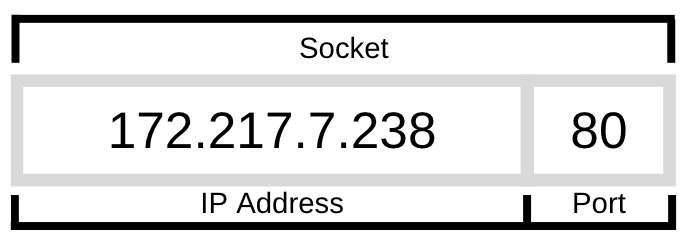
\includegraphics[width=1\linewidth]{00-images/15-socket_address.png}
    \caption{Soket Adresi}
    \label{fig:my_label}
\end{figure}

% ///////////////////////////////////////////////////////////////////

\section{TCP Soket Server ve Client}

\begin{question}
TCP Soket kullanılarak Kullanıcı\textbf{(Client)} tarafından input olarak alınan tek seferlik mesajın Sunucuya\textbf{(Server)} aktarılmasını sağlıyan sistem için:
	\\ a) Uygun TCP Socket Serveri Tasarlayınız.
	\\ b) Uygun TCP Socket Clienti Tasarlayınız. 
\end{question}

a) TCP Socket Server
\vspace{2mm}
\lstinputlisting[language=Go]{codes/11-tcp_socket_server.go }
\captionof{table}{TCP Soket Server}

b) TCP Socket Client
\vspace{2mm}
\lstinputlisting[language=Go]{codes/11-tcp_socket_server.go }
\captionof{table}{TCP Soket Client}

% ///////////////////////////////////////////////////////////////////

\section{TCP Socketi Ile Surekli İletişim Sağlanması}

\begin{question}
TCP Socket kullanılarak Tek Kullanıcı\textbf{(Client)} tarafından input olarak alınan ve bağlantı süresince birden fazla gönderilebilen mesajın Sunucu\textbf{(Server)} tarafından sürekli olarak karşılanmasını sağlayan sistem için:
	\\ a) Uygun TCP Socket Serveri Tasarlayınız.
	\\ b) Uygun TCP Socket Clienti Tasarlayınız.
\end{question}


a) TCP Socket Server
\lstinputlisting[language=Go]{codes/12-tcp_socket_server.go }
\captionof{table}{TCP Soket Server}

b) TCP Socket Client
\lstinputlisting[language=Go]{codes/12-tcp_socket_server.go }
\captionof{table}{TCP Soket Client}

% ///////////////////////////////////////////////////////////////////
\vspace{20mm}

\section{TCP Socket Serverin Goroutinelerle Birden Fazla Clienti Karsilamasi}

\begin{question}
TCP Socket kullanılarak birden fazla Kullanıcı\textbf{(Client)} tarafından input olarak alınan ve bağlantı süresince birden fazla gönderilebilen mesajın Sunucu\textbf{(Server)} tarafından sürekli olarak karşılanmasını sağlayan sistem için:
	\\ a) Uygun TCP Socket Serveri Tasarlayınız.
	\\ b) Uygun TCP Socket Clienti Tasarlayınız.
\end{question}

a) TCP Socket Server
\lstinputlisting[language=Go]{codes/13-tcp_socket_server.go }
\captionof{table}{TCP Soket Server}

b) TCP Socket Client
\lstinputlisting[language=Go]{codes/13-tcp_socket_server.go }
\captionof{table}{TCP Soket Client}

% ///////////////////////////////////////////////////////////////////

\section{UDP Socketi}

\begin{question}
UDP Soket kullanılarak Kullanıcı\textbf{(Client)} tarafından input olarak alınan tek seferlik mesajın Sunucuya\textbf{(Server)} aktarılmasını sağlıyan sistem için:
	\\ a) Uygun UDP Socket Serveri Tasarlayınız.
	\\ b) Uygun UDP Socket Clienti Tasarlayınız.  
\end{question}

\lstinputlisting[language=Go]{codes/14-udp_socket_server.go }
\captionof{table}{UDP Soket Server}

\lstinputlisting[language=Go]{codes/14-udp_socket_client.go }
\captionof{table}{UDP Soket Client}

% ///////////////////////////////////////////////////////////////////

\section{UDP Socket Servera Çoklu Client Bağlantısı}

\begin{question}
UDP Socket kullanılarak birden fazla Kullanıcı\textbf{(Client)} tarafından input olarak alınan ve birden fazla gönderilebilen mesajın Sunucu\textbf{(Server)} tarafından sürekli olarak karşılanmasını sağlayan sistem için:
	\\ a) Uygun UDP Socket Serveri Tasarlayınız.
	\\ b) Uygun UDP Socket Clienti Tasarlayınız. 
\end{question}


\lstinputlisting[language=Go]{codes/15-udp_socket_server.go }
\captionof{table}{UDP Soket Server}

\lstinputlisting[language=Go]{codes/15-udp_socket_client.go }
\captionof{table}{UDP Soket Client}

% ///////////////////////////////////////////////////////////////////
% needs to be fixed
% \section{UDP Socketi Uzerinden Guvenli Veri Akisi Saglanmasi }

% \begin{question}
% UDP Socket Kullanılarak Veri Aktarımı İçin:
% 	\\ a) Server .
% 	\\ b) Client . 
% \end{question}

% \lstinputlisting[language=Go]{00-codes/16-udp_socket_server.go }
% \captionof{table}{UDP Soket Server}

% \lstinputlisting[language=Go]{00-codes/16-udp_socket_client.go }
% \captionof{table}{UDP Soket Client}

% ///////////////////////////////////////////////////////////////////

\section{Port Taramasi}

\begin{question}
Sistemde açık olarak bulunan portların taranması için:
	\\ a) Uygun TCP Port Taraması Sciptini Yazınız.
	\\ b) Uygun UDP Port Taraması Sciptini Yazınız. 
\end{question}

\lstinputlisting[language=Go]{codes/17-port_scanner.go }
\captionof{table}{UDP ve TCP Port Taraması}


% ///////////////////////////////////////////////////////////////////
% needs to be fixed
% \section{TCP Proxy Server Olusturulmasi}

% \begin{question}
% TCP Proxy:
% 	\\ a) Server .
% \end{question}

% \lstinputlisting[language=Go]{00-codes/18-proxy_server.go }

% \captionof{table}{TCP Proxy Server}

% ///////////////////////////////////////////////////////////////////

\chapter{Soket Programlama Uygulamaları}


% %%%%%%%%%%%%%%%%%%%%%%%%%%%%%%%%%%%%%%%%%
% Engineering Calculation Paper
% LaTeX Template
% Version 1.0 (20/1/13)
%
% This template has been downloaded from:
% http://www.LaTeXTemplates.com
%
% Original author:
% Dmitry Volynkin (dim_voly@yahoo.com.au)
%
% License:
% CC BY-NC-SA 3.0 (http://creativecommons.org/licenses/by-nc-sa/3.0/)
%
%%%%%%%%%%%%%%%%%%%%%%%%%%%%%%%%%%%%%%%%%

%----------------------------------------------------------------------------------------
%	PACKAGES AND OTHER DOCUMENT CONFIGURATIONS
%----------------------------------------------------------------------------------------


\setlength{\headheight}{80pt} % Increase the size of the header to accommodate meta-information
\pagestyle{fancy}\fancyhf{} % Use the custom header specified below
\renewcommand{\headrulewidth}{0pt} % Remove the default horizontal rule under the header

\setlength{\parindent}{0cm} % Remove paragraph indentation
\newcommand{\tab}{\hspace*{2em}} % Defines a new command for some horizontal space

\newcommand\BackgroundStructure{ % Command to specify the background of each page
\setlength{\unitlength}{1mm} % Set the unit length to millimeters

\setlength\fboxsep{0mm} % Adjusts the distance between the frameboxes and the borderlines
\setlength\fboxrule{0.5mm} % Increase the thickness of the border line
\put(10, 10){\fcolorbox{black}{blue!10}{\framebox(155,247){}}} % Main content box
\put(165, 10){\fcolorbox{black}{blue!10}{\framebox(37,247){}}} % Margin box
\put(10, 262){\fcolorbox{black}{white!10}{\framebox(192, 25){}}} % Header box
\put(175, 263){
\includegraphics[height=23mm,keepaspectratio]{00-images/00-logo.png}} % Logo box - maximum height/width: 
}

%----------------------------------------------------------------------------------------
%	HEADER INFORMATION
%-------------------------------------------------------------------------------------

\fancyhead[L]{\begin{tabular}{l r | l r} % The header is a table with 4 columns
\textbf{Ağ Programlama} & Lab. Uygulamları & \textbf{Sayfa} & \thepage/\pageref{LastPage} \\ % Project name and page count
\textbf{Tarih}  & \today \\ % Job number and last updated date
\textbf{Dönemi} & 2022-2023 Bahar & \textbf{Tarih} &\today \\ % Version and reviewed date
\textbf{Ders Sor.} & Prof.Dr.Resul Daş & \textbf{Lab.Sor} & Arş.Gör. Oğuzhan Katar\\ % Designer and reviewer
\end{tabular}}

%-------------------------------------------------------------------------------------
\begin{document}

\AddToShipoutPicture{\BackgroundStructure} % Set the background of each page to that specified above in the header information section

%----------------------------------------------------------------------------------------
%	DOCUMENT CONTENT
%----------------------------------------------------------------------------------------
\section{Go Lang Programlamaya Giriş}
\subsection{Hedefler}
\begin{itemize}
    \item Go dili ile soket programlama uygulamaları yapabilemek.
    \item Go dili ile soket programlama uygulamaları yapabilemek.
\end{itemize}


\subsection{Arka Plan / Senaryo}
Mobil tabanlı bir oyun içerisinde farrklı kullanıcıları bulunan ve joystic ile oynayacaktır. Bunun için soket programlama altyapısı tasarlanacaktır. ..





%----------------------------------------------------------------------------------------

\end{document}
% 
% \renewcommand{\bibname}{Kaynaklar}
%\bibliographystyle{apalike}
\bibliographystyle{plain}
\bibliography{references}


\begin{footnotesize}
\begin{singlespacing}

\end{singlespacing}
\end{footnotesize}



%\newpage





% \begin{sheet}
%     \AddToShipoutPicture{\BackgroundStructure} % Set the background of each page to that specified above in the header information section
%     \section{Go Lang Programlamaya Giriş}
\subsection{Hedefler}
\begin{itemize}
    \item Go dili ile soket programlama uygulamaları yapabilemek.
    \item Go dili ile soket programlama uygulamaları yapabilemek.
\end{itemize}


\subsection{Arka Plan / Senaryo}
Mobil tabanlı bir oyun içerisinde farrklı kullanıcıları bulunan ve joystic ile oynayacaktır. Bunun için soket programlama altyapısı tasarlanacaktır. ..


% \end{sheet}

%----------------------------------------------------------------------------------------
%	DOCUMENT CONTENT
%----------------------------------------------------------------------------------------




\begin{footnotesize}
\begin{singlespacing}
\bibliographystyle{ieeetr}
\bibliography{references}
\end{singlespacing}
\end{footnotesize}


%\titleformat{\section}[hang]{\normalsize\bfseries\scshape}{\thesection}{0.25cm}{\normalsize\bfseries\scshape}
\titlespacing*{\section}{0pt}{\parskip}{4mm}

\chapter*{Ekler}
\addcontentsline{toc}{section}{\scshape\footnotesize Ekler}
\thispagestyle{empty}
\mathleft


\begin{justify}
\begin{small}
	\setlength{\parindent}{1cm}
	\hspace*{1cm}
\section*{EK-1 Moleküler Dinamik Temel Algoritması}	

%----------------------------------------------------------------------------------------------------
%----------------------------------------------------------------------------------------------------
%				 EK METİNİNİ GİRİNİZ !
%----------------------------------------------------------------------------------------------------
%----------------------------------------------------------------------------------------------------

\newpage
\section*{EK-2: Gömülü Atom Metodu Parametrelerinin Optimizasyonu}

\newpage
\section*{EK-3: Ovıto Görselleştirme ve Analiz Programının Kullanımı}

\newpage


\end{small}
\end{justify}
 % Ekler listeniz yoksa lütfen bu komudu pasif pozisyona getiriniz!
\chapter*{Özgeçm\.{i}ş}
\thispagestyle{empty}
\addcontentsline{toc}{section}{\scshape\footnotesize Özgeçmiş}

%----------------------------------------------------------------------------------------
%	BU BÖLÜM ÖZGEÇMİŞ METNİNİN BULUNDUĞU YERDİR. BU ŞABLON KULLANILARAK KENDİ ÖZGEÇMİŞİNİZİ OLUŞTURABİLİRSİNİZ.
%  NOT: Size ait olmayan bilgileri mutlaka siliniz...
%----------------------------------------------------------------------------------------

\begin{center}

\hspace{0cm}{\textbf{\tezyazari}}\\
%\vspace{0.35cm}
\end{center}
\setlength{\tabcolsep}{20pt}
\renewcommand{\arraystretch}{0.5}

\begin{table}[ht!]
\setlength{\tabcolsep}{20pt}
\renewcommand{\arraystretch}{1}
\begin{center}
\begin{tabular}{p{0.27\textwidth} p{0.5\textwidth}}
\footnotesize\textbf{{KİŞİSEL BİLGİLER}} \\
\cmidrule[0.1mm]{1-2} 
\hspace{0.5cm}\textbf{\raggedright \footnotesize Doğum Yeri}						& \hspace{-2cm}\footnotesize : Bursa\\
\hspace{0.5cm}\textbf{\raggedright \footnotesize Doğum Yılı}						& \hspace{-2cm}\footnotesize : 1994 \\
\hspace{0.5cm}\textbf{\raggedright \footnotesize Uyruğu}							& \hspace{-2cm}\footnotesize : T.C.\\
\hspace{0.5cm}\textbf{\raggedright \footnotesize Adres}							& \hspace{-2cm}\footnotesize : Üniversite Mahallesi Yahya Kemal Caddesi No:24/A Merkez/ELAZIĞ\\
\hspace{0.5cm}\textbf{\raggedright \footnotesize E-posta}							& \hspace{-2cm}\footnotesize : ugur.firat.education@gmail.com	\\
\hspace{0.5cm}\textbf{\raggedright \footnotesize Yabancı Diller}					& \hspace{-2cm}\footnotesize : İngilizce(C2)\\
\cmidrule[0.1mm]{1-2}\vspace{0.1cm}

\footnotesize\textbf{{EĞİTİM BİLGİLERİ}} \\
\cmidrule[0.1mm]{1-2} 
\hspace{0.5cm}\textbf{\raggedright \footnotesize Lisans}						& \hspace{-2cm}\footnotesize : Vilniaus Kolegija/University of Applied Sciences, Software Engineering, 2019 - 2020\\
\hspace{0.5cm}\textbf{\raggedright \footnotesize Lisans}						& \hspace{-2cm}\footnotesize : Fırat Üniversitesi, Teknoloji Fakültesi, Yazılım Mühendisliği Bölümü, 2015 - 2022\\
\cmidrule[0.1mm]{1-2}\vspace{0.1cm}

\footnotesize\textbf{TEKNOLOJİ} &\vspace{0.03cm}\hspace{-2.8cm}\footnotesize\textbf{DENEYİMİ} \\
\cmidrule[0.1mm]{1-2} 
%& \hspace{-2cm}{\footnotesize \textcolor{red}{Buradaki bilgiler gerçekçi olmalıdır, Etik kurallara uyunuz’}}	\\
%\hspace{0.5cm}\raggedright \footnotesize \checkmark						& \hspace{-2cm}\footnotesize : Kullandığınız laboratuvar cihazları, bildiğiniz deney sistemleri gibi bilgiler veriniz\\
\hspace{0.5cm}\raggedright \footnotesize \checkmark						& \hspace{-2cm}\footnotesize Python: \hspace{0.3cm} Flask, PyModbus, Numpy, Pandas, Matplotlib, PyQt5, PyQtGraph, PyCryptodome, Paramiko, \\
\hspace{0.5cm}\raggedright \footnotesize \checkmark						& \hspace{-2cm}\footnotesize Javascript: Svelte, Vue, React, Node, Web3, Express, Sequelize, Axios, Routify, React Native, Framework7\\
\hspace{0.5cm}\raggedright \footnotesize \checkmark						& \hspace{-2cm}\footnotesize  
Go: \hspace{1cm} Goroutines, TCP/UDP Sockets\\
\hspace{0.5cm}\raggedright \footnotesize \checkmark						& \hspace{-2cm}\footnotesize Solidity: \hspace{0.3cm} Ethereum \& Binance Smart Contracts\\
\hspace{0.5cm}\raggedright \footnotesize \checkmark						& \hspace{-2cm}\footnotesize
C\#: \hspace{0.94cm} Unity 2d Indie Game Development\\
\hspace{0.5cm}\raggedright \footnotesize \checkmark						& \hspace{-2cm}\footnotesize
SQL: \hspace{0.8cm} MySql\\
\cmidrule[0.1mm]{1-2}\vspace{0.1cm}				
\footnotesize\textbf{{İŞ DENEYİMİ}} \\
\cmidrule[0.1mm]{1-2} 
\hspace{0.5cm}\textbf{\raggedright \footnotesize 2018 – 2019}						& \hspace{-2cm}\footnotesize : Web Developer Intern, Vision Factory, Barcelona/ES\\
\hspace{0.5cm}\textbf{\raggedright \footnotesize 2020 – 2021}						& \hspace{-2cm}\footnotesize : PLC Software Developer, Gani Otomasyon, Bursa/TR\\
\hspace{0.5cm}\textbf{\raggedright \footnotesize 2021 – 2022}						& \hspace{-2cm}\footnotesize : Full Stack Web Developer, Arniva Yazılım, Muğla/TR\\
\cmidrule[0.1mm]{1-2}\vspace{0.1cm}
\begin{comment}

\footnotesize\textbf{AKADEMİK} &\vspace{0.09cm}\hspace{-2.8cm}\footnotesize\textbf{FALİYETLER} \\
&\vspace{-0.2cm}\hspace{-2cm}{\footnotesize \textcolor{red}{(Buradaki Bilgiler Kaynak Gösterimleri ile uyumlu olmalıdır)}}\\
\cmidrule[0.1mm]{1-2} 
\hspace{0.5cm}\textbf{\raggedright \footnotesize Makaleler}			& \hspace{-2cm}:\footnotesize\textcolor{red}{Herhangi bir faaliyet yoksa bu alanlar silinmelidir}\\
\hspace{0.5cm}\textbf{\raggedright \footnotesize 1.}					& \hspace{-2cm}\footnotesize ..........\\
\hspace{0.5cm}\textbf{\raggedright \footnotesize 2.}					& \hspace{-2cm}\footnotesize ..........\\
\hspace{0.5cm}\textbf{\raggedright \footnotesize Bildiriler}			& \hspace{-2cm}\footnotesize :\\
\hspace{0.5cm}\textbf{\raggedright \footnotesize 1.}					& \hspace{-2cm}\footnotesize ..........\\
\hspace{0.5cm}\textbf{\raggedright \footnotesize 2.}					& \hspace{-2cm}\footnotesize ..........\\
\hspace{0.5cm}\textbf{\raggedright \footnotesize Projeler}			& \hspace{-2cm}\footnotesize :\\
\hspace{0.5cm}\textbf{\raggedright \footnotesize 1.}					& \hspace{-2cm}\footnotesize ..........\\
\hspace{0.5cm}\textbf{\raggedright \footnotesize 2.}					& \hspace{-2cm}\footnotesize ..........\\
\end{comment}
\end{tabular}
\end{center}
\end{table}



\newpage

\end{document}

